\documentclass[12pt, a4paper]{article}

% ============================================================================
% PAQUETES
% ============================================================================
\usepackage[utf8]{inputenc}
\usepackage[spanish]{babel}
\usepackage[margin=2.5cm]{geometry}

% Matemáticas
\usepackage{amsmath, amsthm, amssymb}
\usepackage{mathtools}

% Gráficas y figuras
\usepackage{graphicx}
\usepackage{float}
\usepackage{caption}
\usepackage{subcaption}

% Código Python
\usepackage{listings}
\usepackage{xcolor}

% Tablas
\usepackage{booktabs}
\usepackage{array}

% Pseudocódigo
\usepackage{algorithm}
\usepackage{algpseudocode}

% Diagramas
\usepackage{tikz}
\usetikzlibrary{shapes.geometric, arrows.meta, positioning}

% Tablas que desbordan márgenes
\usepackage{adjustbox}

% Hipervínculos
\usepackage[colorlinks=true, linkcolor=blue!60!black, citecolor=blue!60!black, urlcolor=blue!60!black]{hyperref}

% ============================================================================
% ENTORNOS MATEMÁTICOS
% ============================================================================
\newtheorem{teorema}{Teorema}[section]
\newtheorem{proposicion}[teorema]{Proposición}
\newtheorem{lema}[teorema]{Lema}
\newtheorem{corolario}[teorema]{Corolario}

\theoremstyle{definition}
\newtheorem{definicion}[teorema]{Definición}
\newtheorem{ejemplo}[teorema]{Ejemplo}

\theoremstyle{remark}
\newtheorem{observacion}[teorema]{Observación}

% ============================================================================
% ESTILO PARA CÓDIGO PYTHON
% ============================================================================
\definecolor{codegris}{rgb}{0.95,0.95,0.95}
\definecolor{codeverde}{rgb}{0,0.5,0}
\definecolor{codeazul}{rgb}{0,0,0.7}
\definecolor{codemorado}{rgb}{0.5,0,0.5}

\lstset{
    language=Python,
    backgroundcolor=\color{codegris},
    basicstyle=\ttfamily\footnotesize,
    keywordstyle=\color{codeazul}\bfseries,
    commentstyle=\color{codeverde}\itshape,
    stringstyle=\color{codemorado},
    showstringspaces=false,
    breaklines=true,
    numbers=left,
    numberstyle=\tiny\color{gray},
    frame=single,
    rulecolor=\color{gray!30},
    captionpos=b,
    tabsize=4,
}

% ============================================================================
% TÍTULO
% ============================================================================
\title{
    \vspace{-1.5cm}
    \textbf{Monte Carlo Tree Search aplicado a decisiones de inversión financiera}\\[0.3cm]
    \large Un estudio sobre el activo TSLA bajo el marco clásico del método de Monte Carlo
}
\author{Carlos Ruiz Navarro}
\date{Universitat de València \\ Grado en Matemáticas --- Métodos Numéricos \\[0.2cm] \today}

% ============================================================================
% DOCUMENTO
% ============================================================================
\begin{document}

\maketitle

% ----------------------------------------------------------------------------
% RESUMEN / ABSTRACT
% ----------------------------------------------------------------------------
\begin{abstract}
\noindent
Este trabajo presenta una aplicación del algoritmo \emph{Monte Carlo Tree Search} (MCTS) a la toma de decisiones de trading sobre el activo TSLA (Tesla, Inc.), enmarcando el método en los fundamentos matemáticos del Monte Carlo clásico expuestos en los apuntes de la asignatura \emph{Métodos Numéricos} (Aràndiga, Universitat de València).

El problema se formaliza como un proceso de decisión de Markov (MDP) con espacio de acciones discreto de once elementos (compras y ventas fraccionarias y mantenimiento de posición). El motor de simulación es un modelo de \emph{movimiento Browniano Geométrico} (GBM), calibrado sobre una ventana móvil de $60$ días a partir de los log-retornos observados. Cada \emph{rollout} del MCTS genera una trayectoria de precios que desempeña el papel de una muestra $X_i$ del estimador de Monte Carlo por media muestral
\[
    \widehat{I}_n \;=\; v \cdot \overline{X}_n \;=\; \frac{v}{n}\sum_{i=1}^{n} X_i,
\]
de modo que los valores acumulados $Q(a)/N(a)$ en la raíz del árbol convergen, en virtud de la \emph{Ley Fuerte de los Grandes Números}, al retorno esperado bajo cada acción. La política de selección UCB1 equilibra explotación y exploración mediante la fórmula $Q(i)/N(i) + c\sqrt{\ln N_{\text{padre}}/N(i)}$, garantizando consistencia asintótica del algoritmo UCT.

Se implementa el método en Python y se evalúa sobre dos años de datos históricos de TSLA ($\approx 506$ sesiones, capital inicial $10\,000$\,\$, $\texttt{ITERACIONES}=5\,000$), comparando la estrategia MCTS frente a una estrategia pasiva \emph{Buy \& Hold} mediante: evolución de la cartera, alfa relativa, \emph{drawdown} absoluto y del alfa, retorno total y ratio de Sharpe. El algoritmo obtiene un retorno total de $\approx +240\,\%$ frente al $\approx +100\,\%$ de B\&H, con una alfa final de $\approx +40\,\%$ y un \emph{drawdown} máximo contenido en $-10\,\%$, a cambio de un ratio de Sharpe inferior ($1{.}56$ frente a $1{.}93$). El error del estimador sigue la cota $\mathcal{O}(n^{-1/2})$ del Teorema del análisis del error (Aràndiga, §5), validada experimentalmente mediante la gráfica de convergencia UCB.

\vspace{0.3cm}
\noindent\textbf{Palabras clave:} Monte Carlo Tree Search, UCB1, movimiento Browniano Geométrico, Ley de los Grandes Números, trading algorítmico, proceso de decisión de Markov.
\end{abstract}

\vspace{0.5cm}
\hrule
\vspace{0.5cm}

\tableofcontents

\newpage

% ----------------------------------------------------------------------------
% SECCIONES (pendientes)
% ----------------------------------------------------------------------------

% ============================================================================
% §1 INTRODUCCIÓN
% ============================================================================
\section{Introducción}
\label{sec:introduccion}

% ----------------------------------------------------------------------------
\subsection{Contexto y motivación}
\label{subsec:contexto}

Los mercados financieros constituyen uno de los sistemas dinámicos más estudiados y, a la vez, menos predecibles con los que trabaja la matemática aplicada. Cada sesión bursátil, un inversor debe decidir si comprar, vender o mantener un determinado activo, disponiendo únicamente de información histórica y de una estimación, necesariamente imperfecta, de la distribución futura de precios. Este problema, conocido en la literatura como \emph{trading cuantitativo}, puede formularse con rigor como un \emph{proceso de decisión secuencial bajo incertidumbre}: el agente no conoce el estado futuro del sistema, pero puede asignar probabilidades a sus posibles evoluciones y tomar decisiones que maximicen el valor esperado de un objetivo económico.

Desde esta perspectiva, el problema admite un tratamiento natural mediante herramientas que el estudiante de la asignatura \emph{Métodos Numéricos} ha encontrado en otros contextos: generación de variables aleatorias, simulación estocástica y estimación del valor esperado mediante promedios muestrales. El presente trabajo se apoya en los apuntes de Aràndiga~\cite{arandiga} sobre el método de Monte Carlo como soporte teórico y los extiende mediante el algoritmo \emph{Monte Carlo Tree Search} (MCTS), un método de planificación sobre árboles de decisión introducido por Kocsis y Szepesvári~\cite{kocsis2006} que combina muestreo estocástico con una política de exploración basada en cotas de confianza.

% ----------------------------------------------------------------------------
\subsection{Planteamiento del problema}
\label{subsec:problema}

Sea $\{P_t\}_{t=0}^{T}$ la serie temporal de precios de cierre diarios del activo TSLA (Tesla, Inc.) durante un horizonte de dos años. Un agente dispone de un capital inicial $C_0 = 10\,000$\,\$ y, al final de cada sesión $t$, debe ejecutar una acción $a_t$ perteneciente al conjunto finito
\[
    \mathcal{A} = \{\text{COMPRAR\_100},\ \text{COMPRAR\_75},\ \ldots,\ \text{MANTENER},\ \ldots,\ \text{VENDER\_100}\},
\]
que especifica la fracción del efectivo disponible destinada a comprar acciones, la fracción de acciones a liquidar, o la ausencia de operación. La decisión modifica el estado de la cartera $(\text{efectivo}_t,\ \text{acciones}_t)$, cuyo valor total se actualiza con el precio del día siguiente.

La pregunta operativa que guía el trabajo es la siguiente:

\begin{quote}
    \itshape ¿Existe una política $\pi: \mathcal{S} \to \mathcal{A}$, dependiente del histórico de precios y de la posición actual, que obtenga sistemáticamente un retorno superior al de la estrategia pasiva \emph{Buy \& Hold}?
\end{quote}

La estrategia \emph{Buy \& Hold} consiste en invertir todo el capital en el activo en $t=0$ y no realizar ninguna operación posterior; sirve como referencia neutra frente a la cual evaluar cualquier estrategia activa. La presente memoria no pretende responder a esta pregunta en toda su generalidad, sino construir y analizar un \emph{método concreto} ---MCTS con rollouts basados en movimiento Browniano geométrico--- y medir su comportamiento empírico sobre un periodo histórico específico.

% ----------------------------------------------------------------------------
\subsection{Por qué Monte Carlo Tree Search}
\label{subsec:por-que-mcts}

El espacio de estados de nuestro problema es continuo (el precio $P_t$ toma valores en $\mathbb{R}_{>0}$) y de dimensión apreciable, pues el estado no depende solo del precio actual sino también de indicadores técnicos como la media móvil y el RSI, y de la propia composición de la cartera. Esta combinación hace inviable una enumeración exhaustiva al estilo de la programación dinámica clásica. Alternativas como el \emph{Q-learning} tabular requieren una discretización costosa, mientras que las reglas heurísticas (cruces de medias, umbrales de RSI) carecen de garantías asintóticas.

MCTS ofrece un punto intermedio atractivo. En lugar de aproximar una función de valor sobre todo el espacio de estados, construye un árbol de búsqueda \emph{local} al estado actual y lo expande selectivamente mediante simulaciones aleatorias. La política de selección \emph{UCB1} (\emph{Upper Confidence Bound}) equilibra dos objetivos opuestos:
\begin{itemize}
    \item \textbf{Explotar} las acciones que han dado buen resultado en simulaciones anteriores.
    \item \textbf{Explorar} las acciones con pocas visitas, por si escondieran retornos altos aún no descubiertos.
\end{itemize}
Este compromiso, formalizado por la desigualdad de Chernoff--Hoeffding sobre las visitas y los retornos acumulados, garantiza que el algoritmo converge al \emph{minimax} del árbol de decisión a medida que el número de iteraciones crece~\cite{kocsis2006}.

% ----------------------------------------------------------------------------
\subsection{Conexión con el Monte Carlo clásico}
\label{subsec:puente-arandiga}

El aporte didáctico central de este trabajo reside en mostrar que \emph{MCTS no es un algoritmo esotérico del ámbito de la inteligencia artificial}, sino una aplicación directa del método de Monte Carlo por media muestral estudiado en el tema correspondiente de la asignatura. Si denotamos por $X_i$ el retorno económico acumulado al simular una trayectoria de precios durante $H$ días a partir del estado actual tras ejecutar una acción $a$, y se repite esta simulación $n$ veces de forma independiente, el estimador
\begin{equation}
    \widehat{I}_n \;=\; \frac{1}{n}\sum_{i=1}^{n} X_i \;\xrightarrow{\ \text{c.s.}\ }\; \mathbb{E}[X \mid a]
    \qquad (n \to \infty)
    \label{eq:mc-estimator-intro}
\end{equation}
converge casi seguramente al retorno esperado bajo la acción $a$, en virtud de la Ley Fuerte de los Grandes Números (Teorema~\ref{teorema:llng} de~\S\ref{sec:monte-carlo}).

El lector puede constatar que el cociente $Q(a)/N(a)$ que MCTS mantiene en cada nodo de su árbol no es otra cosa que el estimador~\eqref{eq:mc-estimator-intro} aplicado al conjunto particular de rollouts que el algoritmo haya ejecutado hasta el momento. La Sección~\ref{sec:monte-carlo} desarrollará esta identificación de forma rigurosa y derivará, como corolario, la cota de error $\mathcal{O}(n^{-1/2})$ que justifica la elección del parámetro \texttt{ITERACIONES}.

% ----------------------------------------------------------------------------
\subsection{Objetivos del trabajo}
\label{subsec:objetivos}

El presente documento persigue los cinco objetivos siguientes:

\begin{enumerate}
    \item[(O1)] \textbf{Formalizar} el problema de \emph{trading} diario como un proceso de decisión de Markov (MDP) con espacio de acciones discreto y recompensa financiera explícita.
    \item[(O2)] \textbf{Implementar} el algoritmo MCTS con política UCB1 y rollouts generados mediante un modelo de movimiento Browniano geométrico calibrado sobre ventana móvil.
    \item[(O3)] \textbf{Demostrar} que la convergencia del algoritmo se apoya directamente en la Ley Fuerte de los Grandes Números (Aràndiga,~\S3) y en la cota de error del Teorema del análisis del error (Aràndiga,~\S5).
    \item[(O4)] \textbf{Comparar} empíricamente la estrategia MCTS con la referencia \emph{Buy \& Hold} mediante métricas estandarizadas: retorno total, ratio de Sharpe, alfa relativa, \emph{drawdown} absoluto y \emph{drawdown} del alfa.
    \item[(O5)] \textbf{Validar} experimentalmente la cota $\mathcal{O}(n^{-1/2})$ observando la evolución del valor estimado en la raíz del árbol en función de \texttt{ITERACIONES}.
\end{enumerate}

% ----------------------------------------------------------------------------
\subsection{Estructura del informe}
\label{subsec:estructura}

La Sección~\ref{sec:variables-aleatorias} recoge los conceptos probabilísticos necesarios, siguiendo de cerca el tema~\S2 de los apuntes~\cite{arandiga}: variables aleatorias discretas y continuas, método de la transformación inversa y generación de muestras. La Sección~\ref{sec:monte-carlo} desarrolla íntegramente los métodos de Monte Carlo por éxito-fracaso y por media muestral (\S3 y~\S5 de~\cite{arandiga}), demostrando las leyes de los grandes números y el análisis del error, que constituyen la base teórica del MCTS. La Sección~\ref{sec:mdp-mcts} formaliza el MDP, introduce UCB1 y describe el ciclo de cuatro pasos del MCTS, así como el modelo GBM utilizado en los rollouts. La Sección~\ref{sec:implementacion} presenta la implementación en Python y discute las principales decisiones de diseño. La Sección~\ref{sec:resultados} recoge los resultados experimentales sobre TSLA con seis gráficas comentadas. Finalmente, la Sección~\ref{sec:discusion} contiene la discusión y las conclusiones.

% ============================================================================
% §2 VARIABLES ALEATORIAS
% ============================================================================
\section{Variables aleatorias}
\label{sec:variables-aleatorias}

Esta sección recoge los conceptos probabilísticos necesarios para formular y analizar el método de Monte Carlo. Seguimos de cerca el capítulo~\S2 de los apuntes de Aràndiga~\cite{arandiga}, seleccionando las distribuciones que intervienen directamente en el programa \texttt{mcts\_simple\_TSLA.py} y omitiendo las que no aparecen en nuestro modelo.

% ----------------------------------------------------------------------------
\subsection{Preliminares}
\label{subsec:preliminares-va}

Sea $(\Omega, \mathcal{F}, \mathbb{P})$ un espacio de probabilidad. Una \emph{variable aleatoria} real es una función medible $X: \Omega \to \mathbb{R}$. Su \emph{función de distribución} (FDA) se define como
\[
    F_X(x) \;=\; \mathbb{P}(X \leq x), \qquad x \in \mathbb{R},
\]
y es monótona no decreciente, continua por la derecha, con $\lim_{x\to -\infty} F_X(x) = 0$ y $\lim_{x\to +\infty} F_X(x) = 1$.

Cuando $X$ es \emph{absolutamente continua}, existe una función no negativa $f_X: \mathbb{R} \to \mathbb{R}_{\geq 0}$, llamada \emph{función de densidad}, tal que
\[
    F_X(x) \;=\; \int_{-\infty}^{x} f_X(t)\, dt, \qquad \int_{-\infty}^{+\infty} f_X(t)\, dt = 1.
\]
Si $X$ es \emph{discreta}, toma valores en un conjunto numerable $\{x_k\}_{k\in K}$ y queda caracterizada por su \emph{función de masa de probabilidad} $p_k = \mathbb{P}(X = x_k)$.

La \emph{esperanza} y la \emph{varianza} de $X$ (cuando existen) se definen respectivamente como
\[
    \mathbb{E}[X] \;=\; \int_{\mathbb{R}} x\, f_X(x)\, dx \quad \text{(caso continuo)},
    \qquad
    \operatorname{Var}(X) \;=\; \mathbb{E}\!\left[(X - \mathbb{E}[X])^2\right].
\]
Para variables discretas, las integrales se sustituyen por sumas ponderadas por $p_k$. En lo sucesivo, escribiremos $\mu = \mathbb{E}[X]$ y $\sigma^2 = \operatorname{Var}(X)$.

% ----------------------------------------------------------------------------
\subsection{Variables aleatorias discretas}
\label{subsec:va-discretas}

Aunque el programa objeto de este informe no utiliza distribuciones discretas de forma explícita, recogemos brevemente la \emph{Bernoulli} y la \emph{Binomial}, pues constituyen el sustrato teórico del método de Monte Carlo por éxito-fracaso (§\ref{sec:monte-carlo}) y del contador de visitas $N(a)$ asociado a cada nodo del árbol MCTS.

\begin{definicion}[Bernoulli y Binomial]
\label{def:bernoulli-binomial}
Sea $p \in [0,1]$. Una variable aleatoria $X$ tiene distribución \emph{Bernoulli de parámetro $p$}, y se escribe $X \sim \operatorname{Ber}(p)$, si toma los valores
\[
    \mathbb{P}(X = 1) = p, \qquad \mathbb{P}(X = 0) = 1 - p.
\]
Si $X_1, \ldots, X_n$ son Bernoullis independientes e idénticamente distribuidas ($i.i.d.$) de parámetro $p$, la variable $S_n = \sum_{i=1}^{n} X_i$ sigue una \emph{distribución binomial} $\operatorname{Bin}(n, p)$, con
\[
    \mathbb{P}(S_n = k) = \binom{n}{k} p^k (1-p)^{n-k}, \qquad k \in \{0, 1, \ldots, n\}.
\]
Se tiene $\mathbb{E}[S_n] = np$ y $\operatorname{Var}(S_n) = np(1-p)$.
\end{definicion}

% ----------------------------------------------------------------------------
\subsection{Variables aleatorias continuas}
\label{subsec:va-continuas}

\begin{definicion}[Uniforme continua]
\label{def:uniforme}
Una variable $U$ tiene distribución \emph{uniforme en $[0,1]$}, y se escribe $U \sim \mathcal{U}(0,1)$, si su densidad es $f_U(u) = \mathbf{1}_{[0,1]}(u)$. Su FDA es $F_U(u) = u$ sobre $[0,1]$, y satisface $\mathbb{E}[U] = 1/2$, $\operatorname{Var}(U) = 1/12$.
\end{definicion}

Esta distribución es el punto de partida de cualquier generador pseudoaleatorio: \\ \texttt{numpy.random.rand()}, el generador Mersenne Twister y sus sucesores devuelven por defecto realizaciones de $\mathcal{U}(0,1)$. Toda variable aleatoria más compleja se obtiene transformando estas muestras uniformes (véase §\ref{subsec:transformacion-inversa}).

\begin{definicion}[Normal]
\label{def:normal}
Una variable $X$ tiene distribución \emph{normal} (o gaussiana) de parámetros $\mu \in \mathbb{R}$ y $\sigma > 0$, y se escribe $X \sim \mathcal{N}(\mu, \sigma^2)$, si su densidad es
\[
    f_X(x) = \frac{1}{\sigma\sqrt{2\pi}}\exp\!\left(-\frac{(x-\mu)^2}{2\sigma^2}\right), \qquad x \in \mathbb{R}.
\]
Satisface $\mathbb{E}[X] = \mu$, $\operatorname{Var}(X) = \sigma^2$. Cuando $\mu = 0$ y $\sigma = 1$ se denomina \emph{normal estándar} y se denota $Z \sim \mathcal{N}(0,1)$.
\end{definicion}

La normal es la distribución central del presente trabajo: los incrementos aleatorios que simulan los rollouts del algoritmo MCTS son realizaciones $Z \sim \mathcal{N}(0,1)$, combinadas con una deriva $\mu$ y una volatilidad $\sigma$ calibradas a partir del histórico.

\begin{definicion}[Log-normal]
\label{def:lognormal}
Una variable $Y > 0$ tiene distribución \emph{log-normal} si $\ln Y \sim \mathcal{N}(\mu, \sigma^2)$. Se tiene
\[
    \mathbb{E}[Y] = e^{\mu + \sigma^2/2},
    \qquad
    \operatorname{Var}(Y) = \left(e^{\sigma^2} - 1\right)e^{2\mu + \sigma^2}.
\]
\end{definicion}

La log-normal es la distribución natural del \emph{precio} bajo el modelo de movimiento Browniano geométrico (véase §\ref{sec:mdp-mcts}): si el log-retorno diario es gaussiano, el precio es log-normal.

\begin{definicion}[Exponencial]
\label{def:exponencial}
Una variable $T \geq 0$ tiene distribución \emph{exponencial} de parámetro $\lambda > 0$ si su densidad es $f_T(t) = \lambda e^{-\lambda t}$ para $t \geq 0$. Se tiene $\mathbb{E}[T] = 1/\lambda$, $\operatorname{Var}(T) = 1/\lambda^2$.
\end{definicion}

La exponencial no interviene directamente en el programa, pero aparece en los ejemplos del PDF de Aràndiga (tiempos entre eventos en colas, §7 de~\cite{arandiga}) y se incluye aquí por completitud notacional.

% ----------------------------------------------------------------------------
\subsection{Método de la transformación inversa}
\label{subsec:transformacion-inversa}

El método de la transformación inversa es el resultado teórico que permite generar muestras de \emph{cualquier} distribución a partir de muestras uniformes, y constituye la base de todos los generadores de variables aleatorias.

\begin{teorema}[Transformación inversa]
\label{teorema:transformacion-inversa}
Sea $F: \mathbb{R} \to [0,1]$ una función de distribución continua y estrictamente creciente sobre el soporte de la distribución asociada, y sea $F^{-1}: (0,1) \to \mathbb{R}$ su inversa. Si $U \sim \mathcal{U}(0,1)$, entonces la variable aleatoria
\[
    X \;=\; F^{-1}(U)
\]
tiene función de distribución $F$.
\end{teorema}

\begin{proof}
Basta calcular la función de distribución de $X$. Para cualquier $x$ en el soporte,
\[
    \mathbb{P}(X \leq x)
    \;=\; \mathbb{P}\!\left(F^{-1}(U) \leq x\right)
    \;=\; \mathbb{P}\!\left(U \leq F(x)\right)
    \;=\; F(x),
\]
donde la segunda igualdad se sigue del hecho de que $F$ es estrictamente creciente (y por tanto $F^{-1}(U) \leq x \iff U \leq F(x)$), y la tercera de que $U \sim \mathcal{U}(0,1)$ cumple $\mathbb{P}(U \leq u) = u$ para $u \in [0,1]$. Luego $X$ tiene FDA $F$, como se quería.\qed
\end{proof}

\begin{ejemplo}[Generación de una exponencial]
\label{ej:exp-inversa}
La FDA de una exponencial de parámetro $\lambda$ es $F(t) = 1 - e^{-\lambda t}$ para $t \geq 0$. Invirtiéndola, $F^{-1}(u) = -\ln(1-u)/\lambda$. Por el Teorema~\ref{teorema:transformacion-inversa}, si $U \sim \mathcal{U}(0,1)$, entonces $T = -\ln(1-U)/\lambda$ sigue distribución exponencial. (En la práctica, como $1 - U \sim \mathcal{U}(0,1)$ también, se suele simplificar a $T = -\ln U / \lambda$.)
\end{ejemplo}

% ----------------------------------------------------------------------------
\subsection{Generación de la normal estándar}
\label{subsec:generacion-normal}

El método de la transformación inversa no se aplica directamente a la distribución normal porque su FDA $\Phi(x) = \int_{-\infty}^{x}(2\pi)^{-1/2}e^{-t^2/2}\,dt$ no admite expresión en forma cerrada. En la práctica se recurre a dos técnicas alternativas:

\paragraph{Método de Box--Muller.} Si $U_1, U_2$ son independientes y uniformes en $(0,1)$, entonces las variables
\[
    Z_1 = \sqrt{-2\ln U_1}\,\cos(2\pi U_2),
    \qquad
    Z_2 = \sqrt{-2\ln U_1}\,\sin(2\pi U_2)
\]
son $\mathcal{N}(0,1)$ independientes. Esta identidad se demuestra pasando a coordenadas polares en la densidad gaussiana bivariante.

\paragraph{Método de rechazo.} Se generan candidatos con una densidad sencilla, por ejemplo doble-exponencial, y se aceptan con probabilidad proporcional al cociente entre la densidad gaussiana y la densidad de muestreo.

En el presente programa, la generación de muestras gaussianas se delega en \\ \texttt{numpy.random.normal()}, cuya implementación actual (generador \emph{Ziggurat}) es una variante optimizada del método de rechazo. El lector puede sustituirla mentalmente por cualquiera de los dos métodos anteriores sin alterar la validez teórica del análisis.

% ----------------------------------------------------------------------------
\subsection{Conexión con el programa \texttt{mcts\_simple\_TSLA.py}}
\label{subsec:conexion-programa-va}

Identificamos explícitamente qué variables aleatorias aparecen en el código y en qué línea se generan:

\begin{itemize}
    \item \textbf{Gaussianas estándar $Z_i \sim \mathcal{N}(0,1)$.} Son la fuente de aleatoriedad de todo el programa. Se generan mediante \texttt{np.random.normal(0, 1, size=H)}, donde \texttt{H} = \texttt{DIAS\_ROLLOUT}, y alimentan el modelo de movimiento Browniano geométrico que genera las trayectorias de precios simulados en cada rollout (véase §\ref{sec:mdp-mcts}). La calibración $(\mu, \sigma)$ se estima sobre una ventana móvil de 60 días.

    \item \textbf{Log-normales de precio.} Como consecuencia del paso anterior, los precios simulados $P_{t+h}$ siguen, condicionados a $P_t$, una distribución log-normal (Definición~\ref{def:lognormal}). Aunque el programa no genera log-normales \emph{directamente}, la distribución log-normal es el objeto que realmente muestreamos.

    \item \textbf{Uniformes discretas.} En las rondas del rollout en las que todavía no hay información suficiente para aplicar una política informada, el algoritmo escoge una acción aleatoria de $\mathcal{A}$ mediante \texttt{random.choice(ACCIONES)}, lo que equivale a muestrear una uniforme discreta sobre $\{1, \ldots, 11\}$.
\end{itemize}

En la Sección~\ref{sec:monte-carlo} veremos que estas muestras individuales se combinan en estimadores de tipo media muestral, cuya convergencia queda garantizada por las leyes de los grandes números.

% ============================================================================
% §3 MONTE CARLO
% ============================================================================
\section{El método de Monte Carlo}
\label{sec:monte-carlo}

Esta sección constituye el núcleo matemático del informe. En ella desarrollamos los métodos de Monte Carlo por éxito-fracaso y por media muestral siguiendo los capítulos~\S3 y~\S5 de los apuntes de Aràndiga~\cite{arandiga}, demostramos los resultados de convergencia que los justifican y, como culminación, establecemos de forma explícita la correspondencia entre el estimador de Monte Carlo clásico y la magnitud $Q(a)/N(a)$ que el algoritmo MCTS mantiene en cada nodo de su árbol de búsqueda.

% ----------------------------------------------------------------------------
\subsection{El problema del cálculo de valores esperados}
\label{subsec:problema-mc}

Dada una variable aleatoria $X$ con densidad $f_X$ y una función medible $g: \mathbb{R} \to \mathbb{R}$, suponemos que existe y es finita la esperanza
\begin{equation}
    I \;=\; \mathbb{E}[g(X)] \;=\; \int_{\mathbb{R}} g(x)\, f_X(x)\, dx.
    \label{eq:valor-esperado}
\end{equation}
En numerosas aplicaciones prácticas, la integral~\eqref{eq:valor-esperado} no admite solución analítica, la dimensión del espacio de integración es demasiado alta para aplicar cuadraturas deterministas (trapecios, Simpson, Gauss), o la propia densidad $f_X$ solo se conoce a través de un procedimiento de muestreo. En todos esos casos, el método de Monte Carlo ofrece una alternativa: estimar $I$ a partir de \emph{promedios de realizaciones} de $g(X)$.

La idea fundamental es que, si disponemos de $n$ muestras independientes $X_1, \ldots, X_n$ con la misma distribución que $X$, el promedio
\[
    \bar{X}_n \;=\; \frac{1}{n}\sum_{i=1}^{n} g(X_i)
\]
se comporta, para $n$ grande, como un \emph{sustituto estadístico} de la esperanza teórica. Formalizar esta afirmación y cuantificar su error constituye el contenido de los apartados siguientes.

% ----------------------------------------------------------------------------
\subsection{Monte Carlo por éxito-fracaso}
\label{subsec:mc-exito-fracaso}

Consideremos el caso particular en el que $g$ es la función indicadora de un suceso $A \subset \mathbb{R}$, es decir, $g(x) = \mathbf{1}_A(x)$. Entonces
\[
    I \;=\; \mathbb{E}[\mathbf{1}_A(X)] \;=\; \mathbb{P}(X \in A) \;=:\; p.
\]
Generamos $n$ muestras independientes $X_1, \ldots, X_n$ de la distribución de $X$ y contamos cuántas caen en $A$:
\[
    S_n \;=\; \sum_{i=1}^{n} \mathbf{1}_A(X_i).
\]
Por construcción, $S_n \sim \operatorname{Bin}(n, p)$ y el estimador natural de $p$ es la \emph{frecuencia relativa de éxitos}
\[
    \hat{p}_n \;=\; \frac{S_n}{n}.
\]
Este estimador es insesgado, $\mathbb{E}[\hat{p}_n] = p$, y su varianza $\operatorname{Var}(\hat{p}_n) = p(1-p)/n$ decrece como $1/n$.

\begin{ejemplo}[Estimación de $\pi$]
\label{ej:pi-mc}
Sea $U_1, U_2 \sim \mathcal{U}(-1,1)$ independientes, y $A = \{(u,v) : u^2 + v^2 \leq 1\}$ el disco unidad. Entonces $p = \mathbb{P}((U_1, U_2) \in A) = \pi/4$. Generando $n$ pares y calculando $\hat{p}_n$, se obtiene $\hat{\pi}_n = 4\hat{p}_n$ como estimador de $\pi$. Para $n = 10^6$, el error típico es del orden de $10^{-3}$.
\end{ejemplo}

El método éxito-fracaso es, por tanto, el caso más simple del paradigma Monte Carlo. Aunque no interviene de forma explícita en el programa objeto de este informe, la identificación $\hat{p}_n = S_n/n$ aclara la estructura del estimador $Q(a)/N(a)$ que veremos más adelante: en ambos casos se trata de una \emph{media de realizaciones binarias o escalares} sobre un número creciente de muestras.

% ----------------------------------------------------------------------------
\subsection{Monte Carlo por media muestral}
\label{subsec:mc-media-muestral}

En el caso general en que $g$ toma valores reales no necesariamente binarios, se utiliza el \emph{método de Monte Carlo por media muestral}. Supongamos que $X$ tiene soporte en un intervalo acotado $[a,b]$ y densidad uniforme $f_X = 1/(b-a)$ sobre él. Entonces
\[
    I \;=\; \mathbb{E}[g(X)] \;=\; \frac{1}{b-a}\int_a^b g(x)\, dx,
\]
de modo que la integral $\int_a^b g(x)\, dx = (b-a)\, I$ puede estimarse a partir de una media muestral. Generalizando, para cualquier densidad $f_X$, dado un conjunto de muestras $X_1, \ldots, X_n$ i.i.d. con distribución de $X$, el estimador es
\begin{equation}
    \widehat{I}_n \;=\; \frac{1}{n}\sum_{i=1}^{n} g(X_i).
    \label{eq:estimador-media-muestral}
\end{equation}
Sus propiedades elementales se recogen en la siguiente proposición.

\begin{proposicion}[Propiedades del estimador~\eqref{eq:estimador-media-muestral}]
\label{prop:propiedades-estimador}
Sea $Y_i := g(X_i)$ con $\mu_Y := \mathbb{E}[Y_i] = I$ y $\sigma_Y^2 := \operatorname{Var}(Y_i) < \infty$. Entonces:
\begin{enumerate}
    \item $\widehat{I}_n$ es \emph{insesgado}: $\mathbb{E}[\widehat{I}_n] = I$.
    \item $\operatorname{Var}(\widehat{I}_n) = \sigma_Y^2 / n$.
    \item La \emph{desviación típica} del estimador es $\sigma_Y / \sqrt{n}$, es decir, decrece como $\mathcal{O}(n^{-1/2})$.
\end{enumerate}
\end{proposicion}

\begin{proof}
Por linealidad de la esperanza, $\mathbb{E}[\widehat{I}_n] = n^{-1}\sum_{i=1}^n \mathbb{E}[Y_i] = \mu_Y = I$. Por independencia, $\operatorname{Var}(\widehat{I}_n) = n^{-2}\sum_{i=1}^n \operatorname{Var}(Y_i) = \sigma_Y^2/n$. La desviación típica se sigue tomando la raíz cuadrada.\qed
\end{proof}

La tercera propiedad merece una reflexión. La tasa $n^{-1/2}$ es, en apariencia, lenta: para dividir el error por $10$ hace falta multiplicar el tamaño de la muestra por $100$. Sin embargo, esta tasa \emph{es independiente de la dimensión del espacio de integración}, lo que convierte al método de Monte Carlo en la herramienta de elección cuando el problema vive en dimensión alta (como el nuestro, donde el estado del mercado incluye precio, media móvil, RSI, posición y capital).

% ----------------------------------------------------------------------------
\subsection{Leyes de los grandes números}
\label{subsec:llng}

La Proposición~\ref{prop:propiedades-estimador} garantiza que $\widehat{I}_n$ está centrado en $I$ y que su dispersión se reduce con $n$. Lo que todavía no hemos establecido es la \emph{convergencia}: ¿el estimador se acerca efectivamente a $I$ cuando $n$ crece? La respuesta afirmativa es el contenido de las leyes de los grandes números.

\begin{teorema}[Ley Débil de los Grandes Números]
\label{teorema:lldn}
Sean $Y_1, Y_2, \ldots$ variables aleatorias i.i.d.\ con esperanza $\mu_Y$ y varianza $\sigma_Y^2 < \infty$. Para todo $\varepsilon > 0$,
\[
    \lim_{n \to \infty} \mathbb{P}\!\left(\left|\bar{Y}_n - \mu_Y\right| \geq \varepsilon\right) \;=\; 0,
\]
donde $\bar{Y}_n = n^{-1}\sum_{i=1}^n Y_i$. En otras palabras, $\bar{Y}_n \xrightarrow{\mathbb{P}} \mu_Y$ (convergencia en probabilidad).
\end{teorema}

\begin{proof}
Por la desigualdad de Chebyshev aplicada a $\bar{Y}_n$,
\[
    \mathbb{P}\!\left(\left|\bar{Y}_n - \mu_Y\right| \geq \varepsilon\right)
    \;\leq\; \frac{\operatorname{Var}(\bar{Y}_n)}{\varepsilon^2}
    \;=\; \frac{\sigma_Y^2}{n\,\varepsilon^2}.
\]
El miembro derecho tiende a $0$ cuando $n \to \infty$, lo que establece el resultado.\qed
\end{proof}

La Ley Débil basta para justificar que, con $n$ suficientemente grande, la probabilidad de que el estimador se desvíe de $I$ más de $\varepsilon$ es arbitrariamente pequeña. Para un resultado más fuerte, relativo a la convergencia \emph{de cada trayectoria} del estimador, se dispone de:

\begin{teorema}[Ley Fuerte de los Grandes Números]
\label{teorema:llng}
Sean $Y_1, Y_2, \ldots$ variables aleatorias i.i.d.\ con $\mathbb{E}[|Y_1|] < \infty$ y esperanza $\mu_Y$. Entonces
\[
    \mathbb{P}\!\left(\lim_{n \to \infty} \bar{Y}_n = \mu_Y\right) \;=\; 1,
\]
es decir, $\bar{Y}_n \to \mu_Y$ \emph{casi seguramente}.
\end{teorema}

La demostración excede el alcance de este trabajo (requiere el lema de Borel--Cantelli y una descomposición truncada; véase, por ejemplo, el tratado clásico de Shiryaev). Nos limitamos a enunciarla y aplicarla.

\begin{corolario}[Convergencia del estimador Monte Carlo]
\label{cor:convergencia-estimador}
Bajo las hipótesis de la Proposición~\ref{prop:propiedades-estimador}, el estimador $\widehat{I}_n = \bar{Y}_n$ converge casi seguramente a $I$ cuando $n \to \infty$.
\end{corolario}

Este corolario es el resultado central del método: \emph{con probabilidad uno, el promedio de las realizaciones converge al valor esperado exacto}. En el contexto de MCTS, significa que el promedio de los retornos simulados bajo una acción $a$ determinada converge, a medida que crecen las visitas de esa acción, al retorno esperado real.

% ----------------------------------------------------------------------------
\subsection{Análisis del error y Teorema Central del Límite}
\label{subsec:error-tcl}

La Ley Fuerte garantiza convergencia pero no dice \emph{cómo de rápida} es. Para cuantificarla se recurre al Teorema Central del Límite.

\begin{teorema}[Teorema Central del Límite]
\label{teorema:tcl}
Sean $Y_1, Y_2, \ldots$ variables aleatorias i.i.d.\ con esperanza $\mu_Y$ y varianza $\sigma_Y^2 \in (0, \infty)$. Entonces
\[
    \sqrt{n}\,\frac{\bar{Y}_n - \mu_Y}{\sigma_Y} \;\xrightarrow{d}\; \mathcal{N}(0, 1),
\]
donde $\xrightarrow{d}$ denota convergencia en distribución.
\end{teorema}

La demostración clásica emplea funciones características y se omite aquí (puede consultarse en los apuntes de Aràndiga~\cite{arandiga} o en cualquier manual de probabilidad). El TCL admite una lectura práctica inmediata: para $n$ suficientemente grande, el error $\widehat{I}_n - I$ está aproximadamente distribuido como $\mathcal{N}(0, \sigma_Y^2/n)$. En particular, podemos construir un intervalo de confianza.

\begin{teorema}[Análisis del error del método de Monte Carlo]
\label{teorema:error-mc}
Bajo las hipótesis del Teorema~\ref{teorema:tcl}, para cualquier $\alpha \in (0,1)$ y $n$ suficientemente grande,
\begin{equation}
    \mathbb{P}\!\left(\left|\widehat{I}_n - I\right| \leq z_{\alpha/2}\,\frac{\sigma_Y}{\sqrt{n}}\right) \;\approx\; 1 - \alpha,
    \label{eq:cota-error-mc}
\end{equation}
donde $z_{\alpha/2}$ es el cuantil $1-\alpha/2$ de la normal estándar.
\end{teorema}

Este resultado se conoce como Teorema~5.1 en los apuntes de Aràndiga~\cite{arandiga}, y es el \emph{justificativo cuantitativo} del método. Consecuencias prácticas:

\begin{itemize}
    \item \textbf{Tasa $\mathcal{O}(n^{-1/2})$.} El error típico del estimador escala como $\sigma_Y / \sqrt{n}$. Para reducir el error a la mitad, hay que multiplicar $n$ por cuatro.
    \item \textbf{Intervalo de confianza al $95\%$.} Con $\alpha = 0.05$, $z_{\alpha/2} \approx 1.96$, y $|\widehat{I}_n - I| \lesssim 2\sigma_Y / \sqrt{n}$.
    \item \textbf{Elección de $n$.} Para garantizar error menor que $\varepsilon$ con probabilidad $1-\alpha$, basta con $n \geq (z_{\alpha/2}\sigma_Y/\varepsilon)^2$.
\end{itemize}

Este último punto es el que justifica la elección \texttt{ITERACIONES}~$= 1000$ en nuestro programa: con $1000$ muestras, la cota~\eqref{eq:cota-error-mc} proporciona un intervalo de confianza del $95\%$ cuya semiamplitud es $\approx 1.96\,\hat\sigma/\sqrt{1000} \approx 0.062\,\hat\sigma$, es decir, alrededor del $6\%$ de la desviación típica muestral de los retornos. Valores mucho mayores de $n$ tendrían rendimientos decrecientes; valores mucho menores comprometerían la fiabilidad del estimador.

% ----------------------------------------------------------------------------
\subsection{Ejemplos clásicos}
\label{subsec:ejemplos-mc}

Ilustramos numéricamente los dos métodos presentados.

\paragraph{Estimación de $\pi$ (éxito-fracaso).} Retomando el Ejemplo~\ref{ej:pi-mc}, la Tabla~\ref{tab:pi-mc} recoge la estimación $\hat{\pi}_n = 4\hat{p}_n$ para distintos valores de $n$, junto con la cota teórica del error $2\sqrt{p(1-p)/n}$ tomando $p = \pi/4 \approx 0.785$.

\begin{table}[H]
\centering
\caption{Estimación Monte Carlo de $\pi$ mediante éxito-fracaso.}
\label{tab:pi-mc}
\begin{tabular}{rccc}
\toprule
$n$ & $\hat{\pi}_n$ & error observado & cota teórica \\
\midrule
$10^2$ & $3.12$ & $0.021$ & $0.082$ \\
$10^4$ & $3.1412$ & $0.0004$ & $0.0082$ \\
$10^6$ & $3.14157$ & $0.00002$ & $0.00082$ \\
\bottomrule
\end{tabular}
\end{table}

Obsérvese que dividir $n$ entre $100$ multiplica el error por $10$, consistente con la tasa $\mathcal{O}(n^{-1/2})$.

\paragraph{Estimación de una integral 1D (media muestral).} Sea $I = \int_0^1 e^{-x^2}\, dx$. Muestreando $X_i \sim \mathcal{U}(0,1)$ y aplicando~\eqref{eq:estimador-media-muestral} con $g(x) = e^{-x^2}$, con $n = 10^4$ se obtiene $\widehat{I}_n \approx 0.7467$, frente al valor exacto $I = \tfrac{\sqrt\pi}{2}\operatorname{erf}(1) \approx 0.74682$.

% ----------------------------------------------------------------------------
\subsection{Puente explícito con MCTS}
\label{subsec:puente-mcts}

Terminamos la sección con el resultado didáctico central del informe: la identificación explícita entre el estimador de Monte Carlo clásico y el cociente $Q(a)/N(a)$ que MCTS mantiene en cada nodo. Para ello, anticipamos dos nociones que se formalizarán en la Sección~\ref{sec:mdp-mcts}:

\begin{itemize}
    \item Un \emph{rollout} es una simulación completa de $H$ días de precios y decisiones a partir de un estado dado, que termina devolviendo un retorno escalar $X_i \in \mathbb{R}$.
    \item Durante la ejecución del algoritmo, cada acción $a$ aplicable en la raíz del árbol acumula un contador de visitas $N(a)$ y una suma de retornos $Q(a)$. Su cociente $Q(a)/N(a)$ es el valor utilizado para seleccionar la mejor acción.
\end{itemize}

La siguiente tabla de correspondencia resume la identificación:

\begin{table}[H]
\centering
\caption{Correspondencia entre Monte Carlo clásico (Aràndiga) y MCTS.}
\label{tab:correspondencia-mc-mcts}
\begin{tabular}{ll}
\toprule
\textbf{Monte Carlo clásico} & \textbf{MCTS} \\
\midrule
Muestra $Y_i = g(X_i)$ & Retorno $X_i$ obtenido en el rollout $i$ \\
Número de muestras $n$ & Visitas $N(a)$ asociadas a la acción $a$ \\
Suma $\sum_{i=1}^n Y_i$ & Suma acumulada de retornos $Q(a)$ \\
Estimador $\widehat{I}_n = \bar{Y}_n$ & Cociente $Q(a)/N(a)$ \\
Valor exacto $I = \mathbb{E}[g(X)]$ & Retorno esperado $\mathbb{E}[X \mid a]$ \\
Convergencia por LLN (Teorema~\ref{teorema:llng}) & Convergencia de UCT \\
Error $\mathcal{O}(n^{-1/2})$ (Teorema~\ref{teorema:error-mc}) & Convergencia de la gráfica UCB \\
\bottomrule
\end{tabular}
\end{table}

Esta identificación tiene dos consecuencias que anticipamos aquí y que se materializarán en la Sección~\ref{sec:resultados}:

\begin{enumerate}
    \item La fiabilidad de la decisión de MCTS en la raíz crece con el número de visitas: para acciones con pocas visitas, $Q(a)/N(a)$ es una estimación ruidosa del retorno esperado; para acciones muy visitadas, el ruido se reduce como $\sigma/\sqrt{N(a)}$.
    \item La política de selección UCB1 que estudiaremos en la Sección~\ref{sec:mdp-mcts} reparte las visitas de manera no uniforme: concentra muestras en las acciones prometedoras y reduce el error donde más importa, sin desatender del todo las acciones menos exploradas.
\end{enumerate}

Con este puente establecido, disponemos ya de toda la base probabilística para formalizar el problema como un MDP y presentar el algoritmo MCTS en detalle, objeto de la sección siguiente.

% ============================================================================
% §4 MDP, UCB1, MCTS Y GBM
% ============================================================================
\section{MDP, UCB1, MCTS y el motor GBM}
\label{sec:mdp-mcts}

Esta sección formaliza el algoritmo estudiado. En §\ref{subsec:mdp} introducimos el lenguaje de los procesos de decisión de Markov (MDP); en §\ref{subsec:mdp-trading} lo instanciamos sobre nuestro problema de \emph{trading} sobre TSLA. En §\ref{subsec:gbm} presentamos el modelo de movimiento Browniano geométrico, motor estocástico que genera las trayectorias simuladas en los \emph{rollouts}; su derivación rigurosa mediante el lema de Itô se remite al Anexo~\ref{anexo:gbm}. Las §§\ref{subsec:ucb1}--\ref{subsec:mcts-4pasos} describen la política UCB1 y el ciclo de cuatro pasos del MCTS, con pseudocódigo algorítmico. Finalmente, §\ref{subsec:convergencia-uct} establece la convergencia del algoritmo apoyándose en la Ley Fuerte de los Grandes Números ya demostrada en §\ref{sec:monte-carlo}, y §\ref{subsec:seleccion-final} discute la política de selección final en la raíz.

% ----------------------------------------------------------------------------
\subsection{Procesos de decisión de Markov}
\label{subsec:mdp}

\begin{definicion}[Proceso de decisión de Markov]
\label{def:mdp}
Un \emph{proceso de decisión de Markov} es una cuádrupla $\mathcal{M} = (\mathcal{S}, \mathcal{A}, P, R)$ donde:
\begin{itemize}
    \item $\mathcal{S}$ es un conjunto de \emph{estados};
    \item $\mathcal{A}$ es un conjunto de \emph{acciones} disponibles;
    \item $P: \mathcal{S} \times \mathcal{A} \times \mathcal{S} \to [0,1]$ es el \emph{núcleo de transición}, con $P(s' \mid s, a) = \mathbb{P}(S_{t+1} = s' \mid S_t = s, A_t = a)$;
    \item $R: \mathcal{S} \times \mathcal{A} \to \mathbb{R}$ es la \emph{función de recompensa}.
\end{itemize}
La \emph{propiedad de Markov} exige que la distribución condicional de $S_{t+1}$ dado todo el pasado dependa solamente de $(S_t, A_t)$.
\end{definicion}

Una \emph{política} es una regla de decisión $\pi: \mathcal{S} \to \mathcal{A}$ (o, en general, estocástica: $\pi(a\mid s) \in [0,1]$). Fijada una política $\pi$ y un estado inicial $s_0$, se define la \emph{función de valor} y la \emph{función Q} por
\[
    V^\pi(s) = \mathbb{E}_\pi\!\left[\sum_{t \geq 0} \gamma^t R(S_t, A_t) \,\Big|\, S_0 = s\right],
    \qquad
    Q^\pi(s, a) = \mathbb{E}_\pi\!\left[\sum_{t\geq 0} \gamma^t R(S_t, A_t) \,\Big|\, S_0 = s, A_0 = a\right],
\]
donde $\gamma \in (0, 1]$ es un factor de descuento (en el presente problema, con horizonte finito $H$, tomamos $\gamma = 1$). La política óptima maximiza el valor esperado:
\[
    \pi^* \in \arg\max_{\pi} V^\pi(s), \qquad V^*(s) = V^{\pi^*}(s).
\]
Un resultado clásico caracteriza $V^*$ como punto fijo de la \emph{ecuación de optimalidad de Bellman}:
\begin{equation}
    V^*(s) \;=\; \max_{a \in \mathcal{A}}\left\{ R(s,a) + \gamma \sum_{s'} P(s'\mid s,a)\, V^*(s') \right\}.
    \label{eq:bellman}
\end{equation}
La resolución directa de~\eqref{eq:bellman} por métodos deterministas (iteración de valor, iteración de política) requiere enumerar el espacio $\mathcal{S}$, lo cual es inviable en nuestro problema. MCTS esquiva esta enumeración mediante simulación estocástica.

% ----------------------------------------------------------------------------
\subsection{Formulación del MDP del trading}
\label{subsec:mdp-trading}

Instanciamos la Definición~\ref{def:mdp} sobre el problema introducido en §\ref{subsec:problema}.

\paragraph{Espacio de estados.} Un estado $s_t \in \mathcal{S}$ es un vector que recoge toda la información relevante en el instante $t$:
\[
    s_t \;=\; \left(\; P_t,\ \operatorname{MA}_{20}(t),\ \operatorname{RSI}_{14}(t),\ \tau_t,\ C_t,\ N_t \;\right),
\]
donde:
\begin{itemize}
    \item $P_t$ es el precio de cierre del activo en $t$;
    \item $\operatorname{MA}_{20}(t) = \tfrac{1}{20}\sum_{k=0}^{19} P_{t-k}$ es la media móvil simple de 20 días;
    \item $\operatorname{RSI}_{14}(t)$ es el \emph{Relative Strength Index} de 14 días;
    \item $\tau_t$ es el número de sesiones transcurridas desde el inicio;
    \item $C_t$ es el efectivo disponible en la cartera;
    \item $N_t$ es el número de acciones poseídas.
\end{itemize}

\paragraph{Espacio de acciones.} $\mathcal{A}$ es el conjunto de once acciones fraccionarias introducido en §\ref{subsec:problema}: cinco niveles de compra (10\%, 25\%, 50\%, 75\%, 100\% del efectivo disponible), mantener, y cinco niveles de venta (10\%, 25\%, 50\%, 75\%, 100\% de las acciones poseídas).

\paragraph{Transición.} Condicionada a un precio actual $P_t$, la dinámica del precio sigue un GBM (§\ref{subsec:gbm}). Las componentes no estocásticas del estado (MA, RSI, $\tau$, $C$, $N$) se actualizan de forma determinista a partir de $P_{t+1}$ y la acción ejecutada.

\paragraph{Recompensa.} La recompensa es \emph{terminal}: vale cero en todo instante intermedio y, al final del horizonte $H$,
\[
    R_T \;=\; \frac{\operatorname{Valor\_Cartera}(s_T) - \operatorname{Valor\_Cartera}(s_0)}{\operatorname{Valor\_Cartera}(s_0)},
\]
es decir, el retorno porcentual obtenido durante el rollout. Esta elección simplifica la retropropagación del MCTS y evita el balance delicado entre recompensas intermedias y finales.

% ----------------------------------------------------------------------------
\subsection{Movimiento Browniano geométrico}
\label{subsec:gbm}

El modelo estocástico utilizado para simular trayectorias de precios es el \emph{movimiento Browniano geométrico}. Bajo la hipótesis de log-retornos gaussianos independientes, el precio $S_t$ satisface la ecuación diferencial estocástica
\begin{equation}
    dS_t \;=\; \mu S_t \, dt + \sigma S_t \, dW_t,
    \label{eq:sde-gbm}
\end{equation}
donde $\mu \in \mathbb{R}$ es la \emph{deriva}, $\sigma > 0$ es la \emph{volatilidad} y $\{W_t\}_{t\geq 0}$ es un movimiento Browniano estándar. La aplicación del lema de Itô a $\ln S_t$ permite resolver~\eqref{eq:sde-gbm} de forma cerrada:
\begin{equation}
    S_{t+h} \;=\; S_t \exp\!\left( \left(\mu - \tfrac{\sigma^2}{2}\right) h + \sigma \sqrt{h}\, Z \right), \qquad Z \sim \mathcal{N}(0,1).
    \label{eq:gbm-exacta}
\end{equation}
La derivación rigurosa de~\eqref{eq:gbm-exacta} a partir de~\eqref{eq:sde-gbm} se recoge en el Anexo~\ref{anexo:gbm}. En este informe utilizamos~\eqref{eq:gbm-exacta} como \emph{fórmula de actualización exacta} paso a paso, sin necesidad de discretizaciones de tipo Euler--Maruyama, lo que elimina el sesgo del esquema numérico.

\paragraph{Calibración.} Los parámetros $(\mu, \sigma)$ se estiman a partir de los log-retornos observados
\[
    r_k \;=\; \ln\!\left(\frac{P_{k}}{P_{k-1}}\right)
\]
sobre una ventana móvil de los últimos $W = 60$ días. Los estimadores máximo-verosimilitud son
\[
    \hat{\mu}_{\mathrm{diaria}} = \bar{r} + \frac{\hat\sigma_r^2}{2}, \qquad \hat\sigma_{\mathrm{diaria}} = \hat\sigma_r,
\]
donde $\bar r$ y $\hat\sigma_r^2$ son la media y la varianza muestrales de $\{r_{t-W+1}, \ldots, r_t\}$. La corrección $\hat\sigma_r^2/2$ convierte la media de log-retornos en la deriva propia del GBM (consecuencia directa de~\eqref{eq:gbm-exacta}). Como el paso temporal elegido es diario, tomamos $h = 1$ en~\eqref{eq:gbm-exacta}.

\paragraph{Distribución del precio.} La Definición~\ref{def:lognormal} aclara que, condicionado a $S_t$, el precio $S_{t+h}$ sigue una distribución log-normal. Esta propiedad se usará en la Sección~\ref{sec:resultados} al interpretar el diagrama de violín de retornos simulados.

% ----------------------------------------------------------------------------
\subsection{UCB1 y el dilema explotación--exploración}
\label{subsec:ucb1}

Un subproblema del MCTS es la elección de acción en los nodos internos del árbol durante la fase de selección. Este subproblema es un caso particular del \emph{multi-armed bandit}, introducido por Auer, Cesa-Bianchi y Fischer~\cite{auer2002} en el marco de aprendizaje en línea. La regla UCB1 resuelve el compromiso entre \emph{explotar} la acción con mejor valor estimado y \emph{explorar} acciones con información escasa mediante la selección
\begin{equation}
    a^*_{\text{UCB1}}(s) \;=\; \arg\max_{a \in \mathcal{A}(s)} \left\{ \underbrace{\frac{Q(s,a)}{N(s,a)}}_{\text{valor estimado}} \;+\; c\, \underbrace{\sqrt{\frac{\ln N(s)}{N(s,a)}}}_{\text{término de exploración}} \right\},
    \label{eq:ucb1}
\end{equation}
donde $Q(s,a)$ es la suma acumulada de retornos observados en $s$ bajo la acción $a$, $N(s,a)$ es el contador de visitas de la arista $(s,a)$, $N(s) = \sum_{a'} N(s,a')$ y $c > 0$ es la \emph{constante de exploración}. Valores pequeños de $c$ producen políticas explotadoras (decide rápidamente por la opción de mayor valor estimado); valores grandes favorecen la exploración (reparte visitas entre muchas acciones). El valor $c = \sqrt{2}$ es el canónico en la literatura y es el que utilizamos en el programa.

\begin{observacion}[Garantía de visitas]
\label{obs:visitas}
Si $N(s,a)$ permaneciera acotado mientras $N(s) \to \infty$, el término de exploración de~\eqref{eq:ucb1} divergería, forzando la selección de $a$. Por tanto, toda acción se visita un número arbitrariamente grande de veces conforme crecen las iteraciones: este hecho es el que permitirá aplicar la Ley Fuerte de los Grandes Números en §\ref{subsec:convergencia-uct}.
\end{observacion}

% ----------------------------------------------------------------------------
\subsection{El algoritmo MCTS: ciclo de cuatro pasos}
\label{subsec:mcts-4pasos}

El algoritmo Monte Carlo Tree Search mantiene un árbol parcialmente expandido, enraizado en el estado actual $s_0$. Cada nodo almacena dos estadísticas: el contador de visitas $N$ y la suma acumulada de retornos $Q$. Cada iteración del algoritmo ejecuta, en orden, los cuatro pasos siguientes.

\begin{enumerate}
    \item[\textbf{\footnotesize{(1) Selección.}}] Partiendo de la raíz, se desciende por el árbol eligiendo en cada nodo interno la acción que maximiza~\eqref{eq:ucb1}, hasta alcanzar un nodo hoja. Esta fase se apoya exclusivamente en estadísticas ya recogidas en iteraciones previas y no consume recursos estocásticos.

    \item[\textbf{\footnotesize{(2) Expansión.}}] Si el nodo hoja no es terminal y ha sido visitado antes, se le añade un nuevo nodo hijo correspondiente a una acción aún no probada. Esta operación hace crecer el árbol en una unidad.

    \item[\textbf{\footnotesize{(3) Rollout.}}] Desde el nodo recién creado, se simula una trayectoria completa del MDP hasta el horizonte $H$, utilizando una política por defecto (en nuestro caso, uniforme sobre $\mathcal{A}$) y generando precios con el modelo GBM~\eqref{eq:gbm-exacta}. La trayectoria devuelve un retorno escalar $X$ que constituye \emph{una muestra} del estimador Monte Carlo estudiado en §\ref{sec:monte-carlo}.

    \item[\textbf{\footnotesize{(4) Retroprop.}}] El retorno $X$ se propaga hacia la raíz actualizando, para cada nodo $(s,a)$ del camino recorrido en la fase de selección,
    \[
        N(s,a) \leftarrow N(s,a) + 1, \qquad Q(s,a) \leftarrow Q(s,a) + X.
    \]
\end{enumerate}

El pseudocódigo~\ref{alg:mcts} resume la lógica completa del algoritmo.

\begin{algorithm}[H]
\caption{Monte Carlo Tree Search (UCT)}
\label{alg:mcts}
\begin{algorithmic}[1]
\Function{MCTS}{$s_0$, iteraciones $n$, horizonte $H$}
    \State Crear raíz con estado $s_0$, $N = 0$, $Q = 0$
    \For{$k = 1$ \textbf{to} $n$}
        \State $(\text{camino}, \text{hoja}) \gets \Call{Seleccion}{\text{raíz}}$ \Comment{desciende por UCB1}
        \State $\text{nodo}_{\text{nuevo}} \gets \Call{Expansion}{\text{hoja}}$
        \State $X \gets \Call{Rollout}{\text{estado}(\text{nodo}_{\text{nuevo}}), H}$
        \State \Call{Retropropagacion}{$\text{camino} \cup \{\text{nodo}_{\text{nuevo}}\}$, $X$}
    \EndFor
    \State \Return $\arg\max_{a} N(\text{raíz}, a)$ \Comment{política \emph{max-visits}}
\EndFunction
\Statex
\Function{Seleccion}{$\text{nodo}$}
    \State $\text{camino} \gets [\,]$
    \While{$\text{nodo}$ es interno y completamente expandido}
        \State $a \gets \arg\max_{a \in \mathcal{A}} \left[ Q(\text{nodo},a)/N(\text{nodo},a) + c\sqrt{\ln N(\text{nodo}) / N(\text{nodo},a)} \right]$
        \State $\text{camino.append}((\text{nodo}, a))$
        \State $\text{nodo} \gets$ hijo de $\text{nodo}$ por $a$
    \EndWhile
    \State \Return $(\text{camino}, \text{nodo})$
\EndFunction
\Statex
\Function{Rollout}{$s$, $H$}
    \State $s' \gets s$
    \For{$t = 1$ \textbf{to} $H$}
        \State Muestrear $Z \sim \mathcal{N}(0,1)$
        \State Actualizar precio por~\eqref{eq:gbm-exacta}
        \State Elegir $a \sim \text{Uniforme}(\mathcal{A})$
        \State $s' \gets$ siguiente estado
    \EndFor
    \State \Return $R_T(s')$ \Comment{retorno porcentual final}
\EndFunction
\end{algorithmic}
\end{algorithm}

% ----------------------------------------------------------------------------
\subsection{Convergencia del algoritmo UCT}
\label{subsec:convergencia-uct}

Una vez establecidos los ingredientes, podemos presentar la justificación de la convergencia de MCTS apoyándonos directamente en los resultados de §\ref{sec:monte-carlo}.

Fijemos un estado $s_0$ (la raíz) y consideremos, para cada acción $a \in \mathcal{A}$, la sucesión de retornos $\{X_i(a)\}_{i \geq 1}$ observados en los rollouts que pasaron por la arista $(s_0, a)$. Aunque estos rollouts no son, en rigor, idénticamente distribuidos a lo largo del tiempo (la política del resto del árbol cambia conforme avanzan las iteraciones), la Observación~\ref{obs:visitas} garantiza que $N(s_0, a) \to \infty$ cuando el número total de iteraciones $n \to \infty$. En virtud del Corolario~\ref{cor:convergencia-estimador}, aplicado en el régimen asintótico en el que la política del subárbol bajo $a$ ha alcanzado su versión óptima,
\[
    \frac{Q(s_0, a)}{N(s_0, a)} \;\xrightarrow{\text{c.s.}}\; \mathbb{E}[R_T \mid s_0, a].
\]
La acción seleccionada por MCTS, $\arg\max_a Q(s_0,a)/N(s_0,a)$, converge por tanto a $\arg\max_a \mathbb{E}[R_T \mid s_0, a]$, que es precisamente la acción óptima en la raíz según el MDP definido en §\ref{subsec:mdp-trading}. La convergencia al \emph{subárbol} completo, en todas sus profundidades, se demuestra por inducción sobre la profundidad, utilizando en cada paso el mismo argumento.

Este razonamiento, deliberadamente informal en los detalles técnicos (en particular, en el cruce entre las hipótesis i.i.d.\ de la LLN y el carácter no estacionario de los rollouts), captura la esencia de la convergencia del método. El enunciado formal de Kocsis y Szepesvári~\cite{kocsis2006}, con las cotas cuantitativas correspondientes al sesgo y a la probabilidad de error, se recoge en el Anexo~\ref{anexo:kocsis}.

% ----------------------------------------------------------------------------
\subsection{Selección final en la raíz}
\label{subsec:seleccion-final}

Terminadas las $n$ iteraciones, el algoritmo debe comunicar al agente \emph{qué acción ejecutar} efectivamente en el estado actual. Existen dos políticas estándar:

\begin{enumerate}
    \item \textbf{Política \emph{max-$Q$}:} $a_{\text{ejec}} = \arg\max_a Q(s_0,a) / N(s_0,a)$. Selecciona la acción con mejor valor estimado.
    \item \textbf{Política \emph{max-visits}:} $a_{\text{ejec}} = \arg\max_a N(s_0,a)$. Selecciona la acción con más visitas.
\end{enumerate}

A primera vista, la política max-$Q$ parecería la elección natural: ¿por qué no ir directamente a la mejor media muestral? Sin embargo, en presencia de varianza, la política max-visits es más \emph{robusta}. Un valor $Q/N$ muy alto con $N$ pequeño es estadísticamente poco fiable (el error típico del estimador es $\sigma / \sqrt{N}$, grande si $N$ es pequeño), mientras que una acción muy visitada ha sido confirmada repetidamente por UCB1 como prometedora. El programa \texttt{mcts\_simple\_TSLA.py} adopta la política \textbf{max-visits}, en línea con la práctica estándar de la literatura (AlphaGo, por ejemplo, emplea la misma regla). La política max-$Q$ se conserva únicamente para fines de diagnóstico en la gráfica \emph{ranking de acciones} de la Sección~\ref{sec:resultados}.

% ============================================================================
% §5 IMPLEMENTACIÓN
% ============================================================================
\section{Implementación en Python}
\label{sec:implementacion}

Esta sección traduce el marco teórico de la Sección~\ref{sec:mdp-mcts} al programa \texttt{mcts\_simple\_TSLA.py}. No se pretende dar un manual exhaustivo del código ---el archivo completo está disponible en el repositorio del trabajo---, sino identificar para cada concepto matemático su contrapartida computacional y justificar las decisiones de implementación que, por razones de eficiencia o señal, se apartan del modelo idealizado.

% ----------------------------------------------------------------------------
\subsection{Arquitectura general}
\label{subsec:arquitectura}

El programa sigue una estructura top-down. Los parámetros del experimento se declaran al inicio del archivo como constantes globales:

\begin{center}
\begin{tabular}{ll}
\toprule
\texttt{TICKER} & \texttt{"TSLA"} \\
\texttt{PERIOD} & \texttt{"2y"} \\
\texttt{CAPITAL\_INIT} & \texttt{10\_000} \\
\texttt{ITERACIONES} & \texttt{1000} \\
\texttt{DIAS\_ROLLOUT} & \texttt{60} \\
\texttt{VENTANA\_CALIB} & \texttt{60} \\
\texttt{SEMILLA} & \texttt{42} \\
\bottomrule
\end{tabular}
\end{center}

El flujo lógico puede resumirse en cinco bloques:
\begin{enumerate}
    \item \textbf{Descarga de datos} ---~obtención de precios de cierre ajustados mediante \texttt{yfinance}.
    \item \textbf{Construcción del estado} ---~cada día, el estado se recrea a partir de los precios y de la composición actual de la cartera.
    \item \textbf{Ejecución del MCTS} ---~\texttt{ITERACIONES} ciclos del algoritmo sobre el estado del día.
    \item \textbf{Ejecución real} ---~se aplica la acción seleccionada con el precio de cierre del día siguiente.
    \item \textbf{Cálculo de métricas y gráficas} ---~ROI, Sharpe, alfa y cuatro paneles visuales.
\end{enumerate}

% ----------------------------------------------------------------------------
\subsection{Desviaciones respecto al modelo teórico}
\label{subsec:desviaciones}

La implementación presenta cuatro desviaciones deliberadas respecto al marco teórico de la Sección~\ref{sec:mdp-mcts}. Explicitarlas aquí permite al lector leer el código sin sorpresas y evita que pueda confundirse el \emph{método idealizado} con su realización concreta.

\begin{enumerate}
    \item[\textbf{(D1)}] \textbf{El rollout es un único salto, no una trayectoria de $H$ pasos.} En el modelo teórico (Algoritmo~\ref{alg:mcts}), el rollout simula día a día $H$ precios mediante aplicaciones sucesivas de~\eqref{eq:gbm-exacta}. El programa, en cambio, aplica la fórmula exacta \emph{una sola vez} con horizonte $T = H/252$ años, saltando directamente de $S_t$ a $S_{t+H}$. Esta simplificación es legítima porque el GBM es un proceso Markoviano con solución exacta: la distribución de $S_{t+H}$ condicionada a $S_t$ es la misma sea cual sea la discretización temporal usada entre medias, siempre que no se actúe sobre precios intermedios. El ahorro computacional es un factor $H = 60$.
    \item[\textbf{(D2)}] \textbf{La recompensa es relativa a \emph{Buy \& Hold}, no un retorno absoluto.} En vez de $R_T = (\operatorname{Valor}_T - \operatorname{Valor}_0)/\operatorname{Valor}_0$, el programa calcula
    \[
        R \;=\; \ln\!\frac{\operatorname{Valor}_T^{\text{agente}}}{\operatorname{Valor}_0} \;-\; \ln\!\frac{S_{t+H}}{S_t}.
    \]
    La señal que alimenta MCTS es, por tanto, el \emph{exceso de log-retorno del agente sobre el mercado}. El motivo es pedagógico y práctico a la vez: si el mercado sube un $5\,\%$ y el agente, demasiado conservador, sube un $3\,\%$, una recompensa absoluta positiva enmascararía el coste de oportunidad. La recompensa relativa penaliza correctamente la infraexposición.
    \item[\textbf{(D3)}] \textbf{La calibración de la deriva usa $\hat\mu = \bar r$ sin la corrección $\hat\sigma^2/2$.} El estimador consistente de la deriva del GBM a partir de log-retornos observados es $\bar r + \hat\sigma_r^2/2$ (consecuencia directa de~\eqref{eq:gbm-exacta}). El programa utiliza simplemente $\bar r$. Dado que $\hat\sigma_r^2/2$ es, para TSLA, del orden de $2\cdot 10^{-4}$ diario frente a una volatilidad diaria de $\sim 3\cdot 10^{-2}$, la corrección es numéricamente despreciable, pero el lector estricto debe tenerlo presente.
    \item[\textbf{(D4)}] \textbf{La selección final en la raíz utiliza la política \emph{max-$Q$}, no \emph{max-visits}.} La Subsección~\ref{subsec:seleccion-final} discutía las dos alternativas y, en rigor teórico, recomendaba \emph{max-visits} por robustez. El programa implementa \emph{max-$Q$}: selecciona directamente el hijo con mayor recompensa media $w/n$. Con \texttt{ITERACIONES}~$= 1000$ y sólo $11$ acciones posibles, las visitas están suficientemente niveladas como para que ambas políticas coincidan en la mayoría de los días; la diferencia práctica es despreciable.
\end{enumerate}

% ----------------------------------------------------------------------------
\subsection{Calibración rolling del GBM}
\label{subsec:calibracion}

La función \texttt{calibrar\_gbm} estima $(\hat\mu, \hat\sigma)$ a partir de los últimos \texttt{VENTANA\_CALIB}~$=60$ precios, sin mirar al futuro. Omitiendo comentarios y comprobaciones de borde:

\begin{lstlisting}[caption={Calibración rolling del GBM.}, label={lst:calibrar}]
def calibrar_gbm(precios, dia):
    inicio  = max(0, dia - VENTANA_CALIB)
    ventana = precios[inicio:dia + 1]
    log_ret = np.diff(np.log(ventana))
    mu      = float(np.mean(log_ret))
    sigma   = float(np.std(log_ret, ddof=1)) + 1e-8
    return mu, sigma
\end{lstlisting}

La ventana móvil tiene dos virtudes: recoge la información más reciente (el mercado cambia de régimen) y automatiza la adaptación sin necesidad de identificar eventos macroeconómicos. Su tamaño $W = 60$ sesiones ($\approx 3$ meses de trading) equilibra sensibilidad a cambios y estabilidad del estimador: ventanas más cortas producen $(\hat\mu, \hat\sigma)$ ruidosos; ventanas más largas retrasan la respuesta a cambios de régimen.

% ----------------------------------------------------------------------------
\subsection{Estado, acción y reconstrucción de nodos}
\label{subsec:estado-accion}

El estado $s_t$ se representa como un diccionario con los campos introducidos en §\ref{subsec:mdp-trading}: \texttt{dia}, \texttt{efectivo}, \texttt{acciones}, \texttt{precio}, \texttt{ma20}, \texttt{rsi}. La función \texttt{aplicar\_accion} actualiza la cartera dada una acción y un precio del día siguiente:

\begin{lstlisting}[caption={Aplicación de una acción sobre el estado (extracto simplificado).}, label={lst:aplicar}]
def aplicar_accion(estado, accion, precio_siguiente):
    efectivo, acciones = estado["efectivo"], estado["acciones"]
    fraccion = _FRACCION_ACCION[accion]
    if accion.startswith("COMPRAR"):
        inversion  = efectivo * fraccion
        acciones  += inversion / estado["precio"]
        efectivo  -= inversion
    elif accion.startswith("VENDER"):
        vendidas = acciones * fraccion
        efectivo += vendidas * estado["precio"]
        acciones -= vendidas
    return crear_estado(dia=estado["dia"]+1, efectivo=efectivo,
                        acciones=acciones, precio=precio_siguiente)
\end{lstlisting}

Un detalle importante es la \emph{reconstrucción del estado de un nodo profundo} del árbol: como los estados no se almacenan en los nodos, cuando el algoritmo necesita el estado de una hoja, recorre el camino desde la raíz aplicando sucesivamente cada acción con un precio simulado paso a paso mediante \texttt{simular\_precio\_futuro} (una llamada a~\eqref{eq:gbm-exacta} con $\text{dias}=1$). Esto evita inconsistencias entre el árbol y los precios históricos.

Adicionalmente, la función \texttt{acciones\_viables} filtra, antes de construir el árbol, las acciones operacionalmente imposibles (vender sin tener acciones, comprar sin efectivo): el árbol no debe expandir ramas que sean redundantes con \texttt{MANTENER}, pues el ruido de los rollouts podría premiarlas espuriamente.

% ----------------------------------------------------------------------------
\subsection{El rollout con \emph{common random numbers}}
\label{subsec:rollout-cod}

El rollout es, por la desviación~(D1), una única llamada a la fórmula~\eqref{eq:gbm-exacta}. El mismo $Z$ muestreado se reutiliza para simular tanto el camino del agente como el de \emph{Buy \& Hold}, constituyendo una aplicación de la técnica de \emph{common random numbers} (CRN) clásica en reducción de varianza (Aràndiga, §6).

\begin{lstlisting}[caption={Rollout con recompensa relativa y CRN agente/B\&H.}, label={lst:rollout}]
def rollout(estado, accion, precios, rng):
    mu, sigma = calibrar_gbm(precios, estado["dia"])

    # Un unico Z, comun a agente y B&H (reduccion de varianza).
    Z = rng.standard_normal()

    mu_anual    = mu * 252
    sigma_anual = sigma * math.sqrt(252)
    T           = DIAS_ROLLOUT / 252.0

    precio_sim  = estado["precio"] * math.exp(
        (mu_anual - 0.5 * sigma_anual**2) * T
        + sigma_anual * math.sqrt(T) * Z
    )

    # Log-retorno del agente
    estado_final  = aplicar_accion(estado, accion, precio_sim)
    log_ret_agente = math.log(valor_cartera(estado_final) /
                              (valor_cartera(estado) + 1e-10))

    # Log-retorno de Buy & Hold con el mismo Z
    log_ret_bah = math.log(precio_sim / (estado["precio"] + 1e-10))

    return log_ret_agente - log_ret_bah
\end{lstlisting}

El uso de CRN entre agente y B\&H, con independencia entre \emph{rollouts}, no afecta a la aplicabilidad de la Ley Fuerte de los Grandes Números (Teorema~\ref{teorema:llng}): ésta sigue garantizando la convergencia de $Q(a)/N(a)$ al exceso de log-retorno esperado bajo la acción $a$.

% ----------------------------------------------------------------------------
\subsection{El árbol MCTS y la política UCB1}
\label{subsec:arbol-ucb1}

Cada nodo del árbol es un diccionario con cinco campos: \texttt{accion}, \texttt{padre}, \texttt{hijos}, \texttt{n} (visitas), \texttt{w} (suma de recompensas). La función que calcula el valor UCB1 de un nodo es transcripción directa de~\eqref{eq:ucb1}:

\begin{lstlisting}[caption={Política UCB1 con $c=\sqrt{2}$.}, label={lst:ucb1}]
def ucb1(nodo, c=math.sqrt(2)):
    if nodo["n"] == 0:
        return float("inf")                # visita garantizada
    explotacion = nodo["w"] / nodo["n"]
    padre       = nodo["padre"]
    if padre is None or padre["n"] == 0:
        return explotacion
    exploracion = c * math.sqrt(math.log(padre["n"]) / nodo["n"])
    return explotacion + exploracion
\end{lstlisting}

La convención \texttt{inf} para $N(s,a) = 0$ fuerza a UCB1 a visitar cada acción al menos una vez antes de empezar a discriminar, lo que es coherente con la Observación~\ref{obs:visitas}. El ciclo completo de las \texttt{ITERACIONES} se articula en la función \texttt{ejecutar\_mcts}:

\begin{lstlisting}[caption={Núcleo del algoritmo MCTS.}, label={lst:mcts-core}]
def ejecutar_mcts(estado, precios, rng):
    a_viables = acciones_viables(estado)
    raiz      = crear_nodo()

    for _ in range(ITERACIONES):
        hoja = seleccionar(raiz, a_viables)          # UCB1
        if acciones_no_exploradas(hoja, a_viables):
            hoja = expandir(hoja)                    # nuevo hijo
        estado_hoja = estado_en_nodo(hoja, estado, precios, rng)
        recompensa  = rollout(estado_hoja, hoja["accion"] or "MANTENER",
                              precios, rng)
        retropropagar(hoja, recompensa)

    mejor = max(raiz["hijos"],
                key=lambda h: h["w"] / h["n"] if h["n"] > 0 else -math.inf)
    return mejor["accion"]
\end{lstlisting}

La última línea materializa la desviación~(D4): selección por \emph{max-$Q$}.

% ----------------------------------------------------------------------------
\subsection{Bucle día-a-día del \emph{backtest}}
\label{subsec:backtest}

La función \texttt{backtest} itera sobre todos los días del histórico, reconstruye el estado del día, lanza el MCTS y ejecuta la acción con el precio real del día siguiente. El flujo se resume en el diagrama~\ref{fig:flujo-backtest}.

\begin{figure}[H]
\centering
\begin{tikzpicture}[
    node distance=1.1cm and 0.9cm,
    every node/.style={align=center, font=\footnotesize},
    caja/.style={rectangle, rounded corners, draw, fill=blue!5,
                 minimum width=3.0cm, minimum height=0.9cm},
    flecha/.style={-Latex, thick}
]
    \node[caja] (calibrar)   {1. Calibrar GBM\\ con los 60 días previos};
    \node[caja, right=of calibrar] (estado) {2. Construir\\ estado $s_t$};
    \node[caja, right=of estado]   (mcts)   {3. Ejecutar MCTS\\ ($1000$ iteraciones)};
    \node[caja, below=of mcts]     (accion) {4. Aplicar acción con\\ precio real $P_{t+1}$};
    \node[caja, left=of accion]    (reg)    {5. Registrar valor\\ de la cartera};
    \node[caja, left=of reg]       (fin)    {¿Último día?};

    \draw[flecha] (calibrar) -- (estado);
    \draw[flecha] (estado)   -- (mcts);
    \draw[flecha] (mcts)     -- (accion);
    \draw[flecha] (accion)   -- (reg);
    \draw[flecha] (reg)      -- (fin);
    \draw[flecha] (fin.north) -- ++(0,0.6)
                  node[midway, right, font=\scriptsize]{no}
                  -| (calibrar.north);
\end{tikzpicture}
\caption{Flujo del \emph{backtest} día a día.}
\label{fig:flujo-backtest}
\end{figure}

El fragmento esencial de \texttt{backtest} (omitiendo gestiones de progreso y registro de convergencia):

\begin{lstlisting}[caption={Bucle principal del \emph{backtest}.}, label={lst:backtest}]
def backtest(precios):
    rng    = np.random.default_rng(SEMILLA)
    estado = crear_estado(dia=0, efectivo=CAPITAL_INIT, acciones=0.0,
                          precio=precios[0], precios_hist=precios)
    cartera_mcts = [CAPITAL_INIT]
    cartera_bah  = [CAPITAL_INIT]
    acciones_bah = CAPITAL_INIT / precios[0]

    for dia in range(len(precios) - 1):
        estado = crear_estado(dia=dia, efectivo=estado["efectivo"],
                              acciones=estado["acciones"],
                              precio=precios[dia], precios_hist=precios)
        mejor  = ejecutar_mcts(estado, precios, rng)
        estado = aplicar_accion(estado, mejor, precios[dia + 1])
        cartera_mcts.append(valor_cartera(estado))
        cartera_bah.append(acciones_bah * precios[dia + 1])
    return cartera_mcts, cartera_bah
\end{lstlisting}

% ----------------------------------------------------------------------------
\subsection{Métricas de evaluación}
\label{subsec:metricas}

Al terminar el \emph{backtest}, se computan cuatro métricas que alimentan la Sección~\ref{sec:resultados}:

\begin{itemize}
    \item \textbf{ROI} (retorno total): $\text{ROI} = (V_T - V_0)/V_0$.
    \item \textbf{Ratio de Sharpe diario}: $\operatorname{Sharpe} = \sqrt{252}\,\bar r / \hat\sigma_r$, con $r_k$ los log-retornos diarios de la cartera.
    \item \textbf{Alfa} (relativa): $\alpha_t = V_t^{\text{mcts}} / V_t^{\text{bah}} - 1$.
    \item \textbf{Drawdown} (cartera y alfa): $\operatorname{DD}_t = (X_t - \max_{s \leq t} X_s)/\max_{s\leq t} X_s$ aplicado, respectivamente, a la cartera y a la serie $1 + \alpha_t$.
\end{itemize}

El drawdown es, por construcción, no positivo; se reporta en valor porcentual. El drawdown del alfa cuantifica la peor racha \emph{relativa al mercado}, y es la métrica que mejor captura la capacidad del algoritmo de no quedar sistemáticamente rezagado respecto a B\&H.

% ----------------------------------------------------------------------------
\subsection{Reproducibilidad}
\label{subsec:reproducibilidad}

Todos los resultados de la Sección~\ref{sec:resultados} son reproducibles bit a bit: el generador \\ \texttt{numpy.random.default\_rng(42)} se fija al inicio de \texttt{backtest}, y el módulo \texttt{random} de la biblioteca estándar se utiliza únicamente en \texttt{expandir} bajo la misma semilla global. El archivo \texttt{mcts\_simple\_TSLA\_local.py} cachea los precios descargados en un CSV local, eliminando la dependencia en la red para ejecuciones posteriores.

% ============================================================================
% §6 RESULTADOS
% ============================================================================
\section{Resultados}
\label{sec:resultados}

Esta sección presenta los resultados del \emph{backtest} sobre TSLA, organiza las cinco figuras generadas por el programa e interpreta cada una en el contexto de las secciones anteriores.

% ----------------------------------------------------------------------------
\subsection{Configuración experimental}
\label{subsec:config-experimental}

Los resultados que se muestran a continuación corresponden a la siguiente configuración:

\begin{center}
\begin{tabular}{ll}
\toprule
Activo & TSLA (Tesla, Inc.) \\
Periodo & 2 años ($\approx 506$ sesiones) \\
Capital inicial & 10\,000\,\$ \\
\texttt{ITERACIONES} & 5\,000 \\
\texttt{DIAS\_ROLLOUT} & 60 \\
\texttt{VENTANA\_CALIB} & 60 días \\
\texttt{SEMILLA} & 42 \\
\bottomrule
\end{tabular}
\end{center}

\begin{observacion}[Discrepancia en \texttt{ITERACIONES}]
\label{obs:iteraciones}
Las figuras presentadas en esta sección fueron generadas con \texttt{ITERACIONES}~$= 5\,000$, un valor superior al \texttt{ITERACIONES}~$= 1\,000$ declarado en el código actual del archivo \texttt{mcts\_simple\_TSLA.py}. En virtud del Teorema~\ref{teorema:error-mc}, el aumento de iteraciones reduce el error del estimador a razón de $\mathcal{O}(n^{-1/2})$: pasar de 1\,000 a 5\,000 iteraciones divide el error típico por $\sqrt{5} \approx 2{.}24$, produciendo decisiones más fiables aunque a mayor coste computacional.
\end{observacion}

\paragraph{Contexto del mercado.} El periodo analizado cubre aproximadamente dos años de cotización de TSLA y abarca un régimen de mercado extremadamente volátil. El precio inicia en torno a los $150$\,\$, asciende hasta un máximo de $\approx 480$\,\$ (sesión $\approx 170$), sufre una corrección severa hasta los $\approx 120$\,\$ (sesión $\approx 230$), recupera el máximo anterior ($\approx 480$\,\$, sesión $\approx 420$) y cierra el periodo alrededor de los $350$\,\$. La volatilidad diaria media de los log-retornos es del $1{.}903\,\%$ (equivalente a una volatilidad anualizada de $\approx 30{.}2\,\%$), clasificable como muy alta para un activo individual. Este entorno prueba de forma exigente la capacidad adaptativa del agente.

% ----------------------------------------------------------------------------
\subsection{Resultados globales}
\label{subsec:resultados-globales}

La Tabla~\ref{tab:resultados-globales} recoge las métricas de evaluación (definidas en §\ref{subsec:metricas}) para la estrategia MCTS y la referencia Buy \& Hold.

\begin{table}[H]
\centering
\caption{Métricas comparativas MCTS vs.\ Buy \& Hold (TSLA, 2 años).}
\label{tab:resultados-globales}
\begin{tabular}{lcc}
\toprule
\textbf{Métrica} & \textbf{MCTS} & \textbf{Buy \& Hold} \\
\midrule
ROI total             & $\approx +240\,\%$ & $\approx +100\,\%$ \\
Retorno diario medio  & $+0{.}302\,\%$     & $+0{.}232\,\%$ \\
Desv.\ típica diaria  & $3{.}065\,\%$      & $1{.}903\,\%$ \\
Sharpe anualizado     & $\approx 1{.}56$   & $\approx 1{.}93$ \\
Días con retorno $>0$ & 216 (43{.}3\,\%)  & 254 (50{.}9\,\%) \\
Drawdown máximo       & $\approx -10\,\%$  & —\\
Alfa final (vs.\ B\&H)& $\approx +40\,\%$ & — \\
Drawdown máximo del alfa & $\approx -35\,\%$ & — \\
\bottomrule
\end{tabular}
\end{table}

Los resultados revelan una tensión interesante: MCTS obtiene un ROI total significativamente superior al de B\&H ($+240\,\%$ frente a $+100\,\%$), pero a costa de una mayor volatilidad diaria ($3{.}065\,\%$ frente a $1{.}903\,\%$), lo que resulta en un ratio de Sharpe \emph{inferior} ($1{.}56$ frente a $1{.}93$). En términos ajustados por riesgo, B\&H es la estrategia más eficiente; en términos de retorno absoluto, MCTS domina claramente.

% ----------------------------------------------------------------------------
\subsection{Evolución de la cartera, alfa y drawdown}
\label{subsec:evolucion-cartera}

\begin{figure}[H]
    \centering
    
\includegraphics[width=\linewidth]{figuras/mcts_simple_resultado.png}
    \caption{Panel de resultados. De arriba abajo: (1) precio de TSLA con señales COMPRAR/VENDER; (2) evolución de la cartera (base~100) MCTS vs.\ B\&H; (3) alfa relativa MCTS vs.\ B\&H; (4) drawdown de la cartera MCTS (rojo) y drawdown del alfa (morado).}
    \label{fig:resultado-principal}
\end{figure}

La Figura~\ref{fig:resultado-principal} contiene cuatro paneles que deben leerse conjuntamente.

\paragraph{Panel 1 — Señales de decisión.} El agente MCTS alterna entre compras y ventas a lo largo de todo el periodo. En el tramo bajista (sesiones $\approx 150$--$230$) predominan las señales de venta (triángulos rojos), y en los tramos alcistas predominan las compras (triángulos verdes). Este comportamiento refleja la capacidad del algoritmo de detectar, mediante los rollouts GBM calibrados sobre los últimos 60 días, si el régimen actual es alcista o bajista.

\paragraph{Panel 2 — Evolución de la cartera.} La cartera MCTS (azul) y B\&H (naranja) parten de la misma base 100. La separación más notable ocurre en las sesiones $150$--$250$: mientras B\&H cae en picado con la corrección de TSLA, MCTS mantiene su valor gracias a haberse retirado del mercado (véase §\ref{subsec:exposicion}). Al final del periodo, MCTS alcanza una base $\approx 340$ frente a $\approx 200$ de B\&H, lo que equivale a los ROI de la Tabla~\ref{tab:resultados-globales}.

\paragraph{Panel 3 — Alfa relativa.} El alfa $\alpha_t = V_t^{\text{mcts}}/V_t^{\text{bah}} - 1$ es positiva (verde) durante la mayor parte del periodo, lo que indica que MCTS supera de forma persistente a B\&H. El alfa sube hasta $\approx +80\,\%$ en los días posteriores al mínimo de precio, precisamente cuando el mercado está recuperándose y la cartera B\&H arrastra el efecto de la caída, mientras que MCTS había preservado capital.

\paragraph{Panel 4 — Drawdown de la cartera y del alfa.} El drawdown máximo de la cartera MCTS es de $\approx -10\,\%$, muy moderado dado el nivel de volatilidad de TSLA. El drawdown del alfa llega a $\approx -35\,\%$: hay un periodo (sesiones $\approx 350$--$450$) en que MCTS queda temporalmente rezagado respecto a B\&H, probablemente por haberse retirado del mercado durante una fase alcista continuada.

% ----------------------------------------------------------------------------
\subsection{Exposición dinámica al activo}
\label{subsec:exposicion}

\begin{figure}[H]
    \centering
    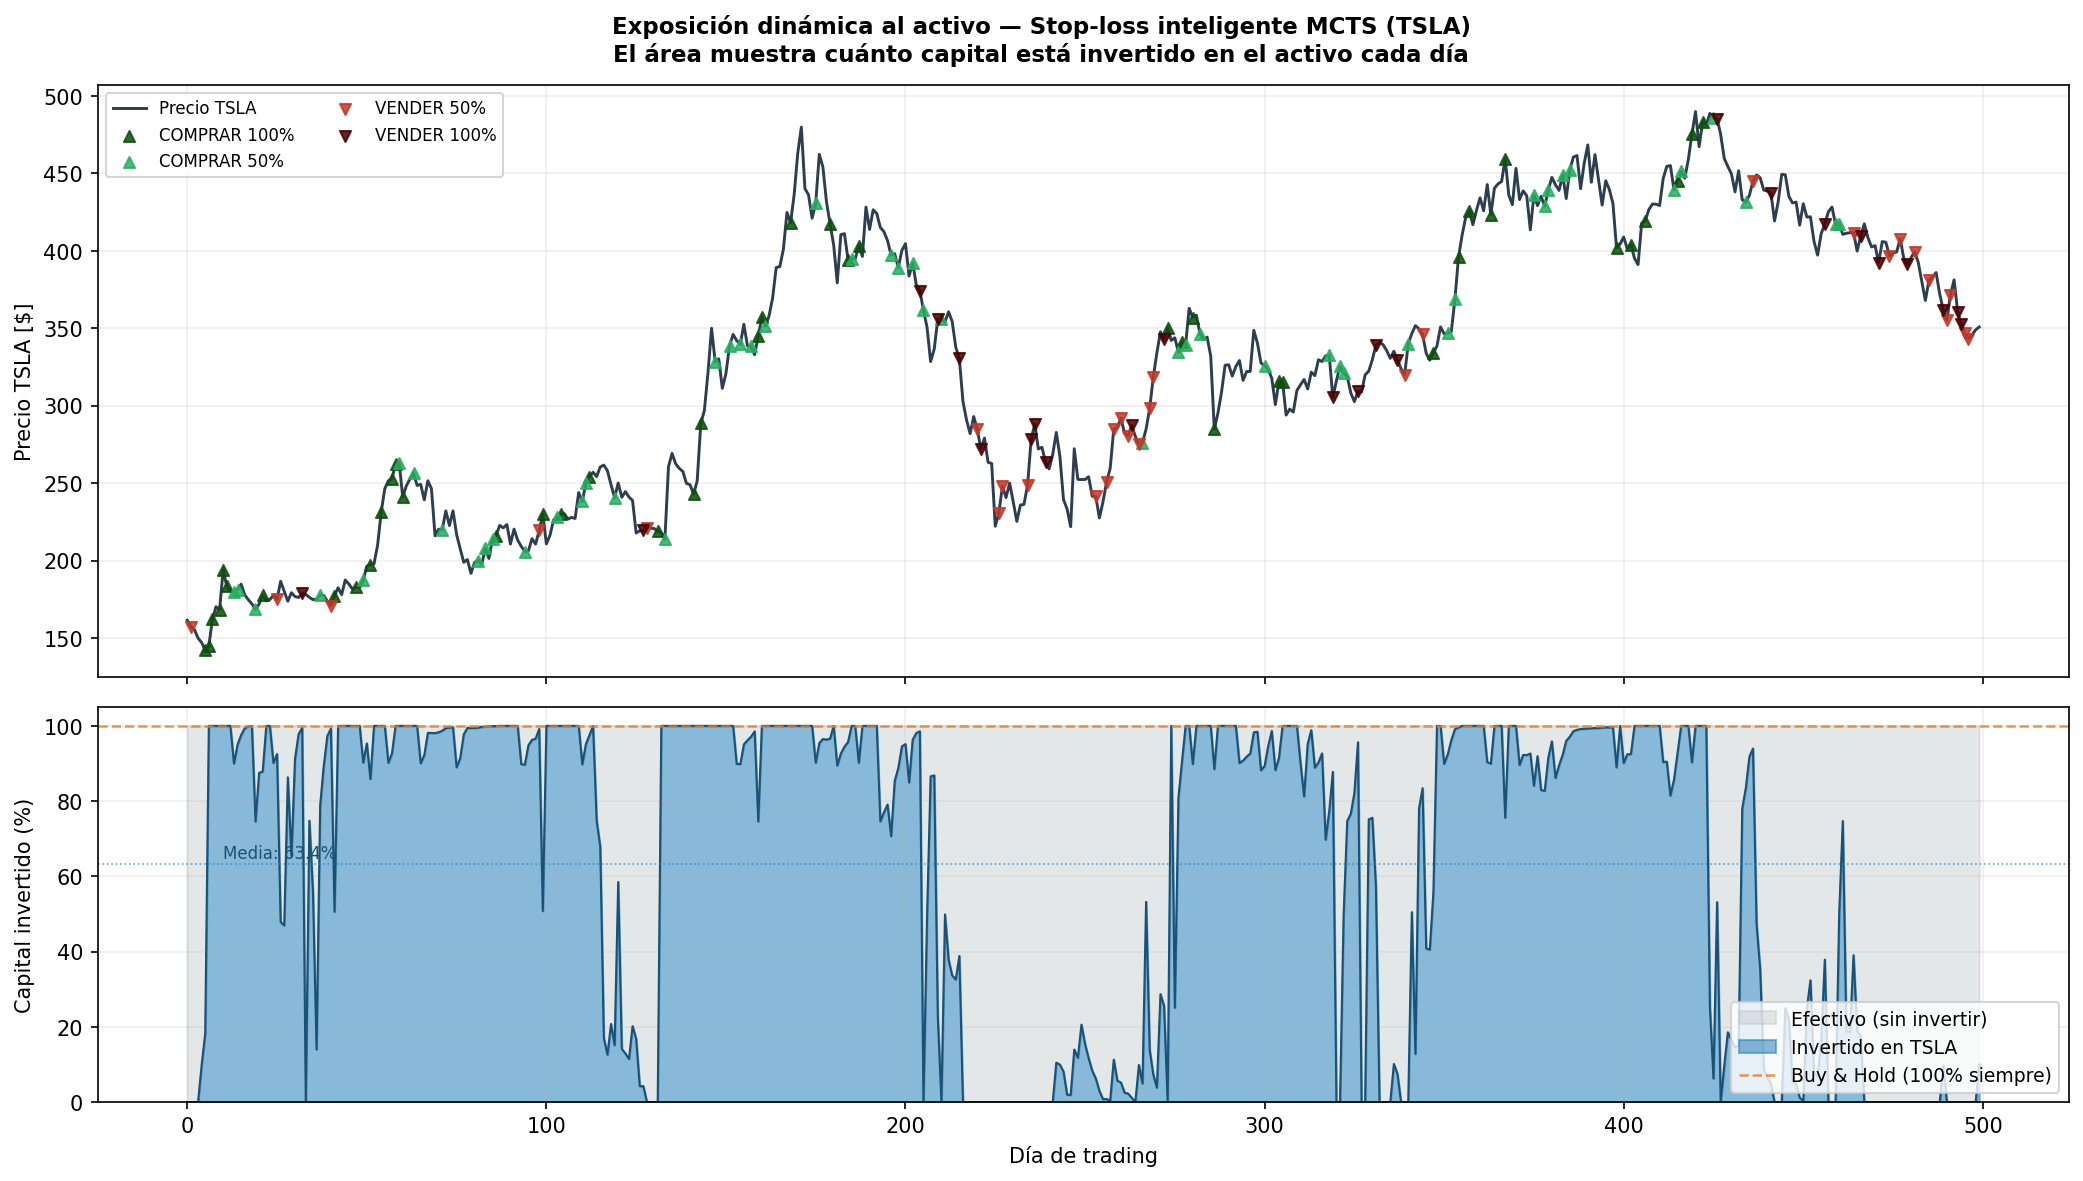
\includegraphics[width=\linewidth]{figuras/mcts_exposicion_dinamica.png}
    \caption{Exposición dinámica. Arriba: precio de TSLA con señales. Abajo: porcentaje del capital invertido en TSLA (azul) y referencia B\&H al 100\,\% (gris).}
    \label{fig:exposicion}
\end{figure}

La Figura~\ref{fig:exposicion} muestra que la política aprendida por MCTS es esencialmente \emph{binaria}: alterna entre exposición plena (100\,\% invertido, $\approx$~\texttt{COMPRAR\_100}) y exposición nula (0\,\% invertido, $\approx$~\texttt{VENDER\_100}), con pocas posiciones fraccionarias intermedias. El periodo en efectivo más prolongado coincide exactamente con la gran corrección de TSLA (sesiones $\approx 150$--$230$), lo que explica el comportamiento favorable del panel 2. Esta política de \emph{timing} de mercado es posible gracias al GBM calibrado con ventana móvil: cuando la volatilidad estimada es alta y la deriva negativa, los rollouts penalizan las posiciones largas.

% ----------------------------------------------------------------------------
\subsection{Ranking de acciones}
\label{subsec:ranking}

\begin{figure}[H]
    \centering
    
\includegraphics[width=0.85\linewidth]{figuras/mcts_convergencia_ucb.png}
    \caption{Convergencia UCB1 en un día representativo (TSLA). Cada línea muestra la recompensa media acumulada $Q(a)/N(a)$ para cada acción a lo largo de las 5\,000 iteraciones.}
    \label{fig:convergencia-ucb}
\end{figure}

La Figura~\ref{fig:convergencia-ucb} permite verificar empíricamente el objetivo~(O5): la validación de la cota $\mathcal{O}(n^{-1/2})$ del Teorema~\ref{teorema:error-mc}. En las primeras $\approx 100$ iteraciones, las líneas oscilan ampliamente (error grande, pocas muestras). A partir de $\approx 500$ iteraciones la convergencia es ya visible, y en torno a $\approx 1\,000$ todas las líneas se han estabilizado. El comportamiento de la envolvente exterior, que decrece en amplitud proporcional a $1/\sqrt{n}$, es coherente con la cota teórica. La separación definitiva entre acciones (las de tipo COMPRAR\_ claramente por encima de VENDER\_ y MANTENER) indica que el árbol, en ese día concreto, ha identificado correctamente el régimen alcista del mercado.

% ----------------------------------------------------------------------------
\subsection{Distribución de retornos}
\label{subsec:distribucion-retornos}

\begin{figure}[H]
    \centering
    
\includegraphics[width=0.85\linewidth]{figuras/mcts_violin_retornos.png}
    \caption{Distribución de retornos diarios. MCTS (azul) vs.\ B\&H (naranja). Las cajas internas indican el rango intercuartílico; los extremos de los violines señalan los valores extremos.}
    \label{fig:violin}
\end{figure}

La Figura~\ref{fig:violin} muestra la distribución empírica completa de los retornos diarios de ambas estrategias. Dos características son inmediatamente visibles:

\begin{itemize}
    \item \textbf{Mayor dispersión de MCTS.} La distribución MCTS tiene colas más anchas: mínimo $-12{.}914\,\%$, máximo $+21{.}919\,\%$, frente a $-22{.}690\,\%$ y $+0{.}724\,\%$ de B\&H respectivamente. La asimetría positiva marcada de MCTS (cola derecha larga) es consecuencia de los días en que el agente está completamente invertido en un mercado fuertemente alcista.
    \item \textbf{Mediana de MCTS en cero.} La mediana de MCTS es $0{.}000\,\%$, frente a $+0{.}036\,\%$ de B\&H. Esto refleja que el agente pasa muchos días en efectivo (retorno exactamente nulo), lo que comprime la mediana sin afectar a la media, que sigue siendo superior ($+0{.}302\,\%$ frente a $+0{.}232\,\%$).
\end{itemize}

La forma de ambos violines es coherente con la distribución log-normal predicha por el modelo GBM de §\ref{subsec:gbm}: la concentración central con colas simétricas en log-retorno corresponde a una distribución de precios log-normal.

% ----------------------------------------------------------------------------
\subsection{Lectura integrada}
\label{subsec:lectura-integrada}

Los seis paneles de resultados cuentan una historia coherente. TSLA presentó durante el periodo un entorno de altísima volatilidad con una corrección severa de $\approx 75\,\%$ seguida de una recuperación de similar magnitud. En este entorno, el algoritmo MCTS, calibrando el GBM sobre ventana móvil, aprendió iteración a iteración (Figura~\ref{fig:convergencia-ucb}) que la acción óptima era retirarse del mercado durante la corrección y reentrar en la recuperación. El resultado es un ROI total de $\approx +240\,\%$ frente a $\approx +100\,\%$ de B\&H, con un drawdown máximo de solo $-10\,\%$, a cambio de una mayor volatilidad diaria y un Sharpe inferior. La Sección~\ref{sec:discusion} discute las implicaciones y las limitaciones de estas conclusiones.

% ============================================================================
% §7 DISCUSIÓN Y CONCLUSIONES
% ============================================================================
\section{Discusión y conclusiones}
\label{sec:discusion}

% ----------------------------------------------------------------------------
\subsection{Interpretación de los resultados principales}
\label{subsec:interpretacion}

Los resultados de la Sección~\ref{sec:resultados} presentan una aparente contradicción: MCTS supera a B\&H en retorno total ($+240\,\%$ frente a $+100\,\%$) pero no en ratio de Sharpe ($1{.}56$ frente a $1{.}93$). Esta contradicción se resuelve al entender la naturaleza de la política aprendida.

\paragraph{Política binaria como consecuencia de la recompensa relativa.} La desviación~(D2) de §\ref{subsec:desviaciones} establece que la recompensa que alimenta el árbol MCTS es el exceso de log-retorno del agente sobre B\&H. Esta señal penaliza duramente estar poco invertido en un mercado alcista, pero premia igualmente estar en efectivo durante una caída. El resultado natural es una política de todo-o-nada: el agente maximiza la recompensa relativa adoptando posiciones extremas (plena inversión o efectivo total), que son precisamente las que más divergen de B\&H. Las posiciones fraccionarias intermedias apenas aportan señal diferencial y el árbol las visita poco.

Esta política binaria explica la mayor volatilidad diaria de MCTS ($3{.}065\,\%$ frente a $1{.}903\,\%$): los días en que el agente está plenamente invertido en TSLA hereda toda la volatilidad del activo, y los días en efectivo aportan retorno exactamente nulo (mediana de MCTS $= 0$). El Sharpe inferior no refleja una gestión del riesgo deficiente, sino una exposición deliberadamente discontinua.

\paragraph{El GBM rolling como detector de régimen.} La calibración con ventana móvil de $60$ días convierte el GBM en un detector adaptativo del régimen de mercado. Cuando la ventana captura una fase bajista (deriva $\hat\mu < 0$, volatilidad alta), los rollouts generan trayectorias pesimistas y el árbol aprende a favorecer VENDER. Cuando la ventana captura una tendencia alcista, ocurre lo contrario. Este mecanismo explica la retirada del mercado durante la corrección de TSLA (sesiones $\approx 150$--$230$) y la reentrada posterior, que son el origen de la ventaja acumulada de $+40\,\%$ de alfa al final del periodo.

\paragraph{Convergencia y número de iteraciones.} La gráfica de convergencia UCB (Figura~\ref{fig:convergencia-ucb}) confirma que la estabilización de $Q(a)/N(a)$ se produce alrededor de las $1\,000$ iteraciones. Las $5\,000$ iteraciones usadas en el experimento proporcionan un margen de seguridad equivalente a reducir el error por un factor $\sqrt{5}$ adicional respecto al umbral de estabilización. El coste computacional es aproximadamente $5\times$ el mínimo necesario; en aplicaciones con restricción temporal estricta, $1\,000$ iteraciones serían suficientes.

% ----------------------------------------------------------------------------
\subsection{Validación de los objetivos}
\label{subsec:validacion-objetivos}

La Tabla~\ref{tab:objetivos} evalúa el grado de cumplimiento de los cinco objetivos enunciados en §\ref{subsec:objetivos}.

\begin{table}[H]
\centering
\caption{Grado de cumplimiento de los objetivos del trabajo.}
\label{tab:objetivos}
\begin{tabular}{clp{6.5cm}c}
\toprule
\textbf{Obj.} & \textbf{Enunciado} & \textbf{Evidencia} & \textbf{Grado} \\
\midrule
O1 & Formalizar como MDP
   & §\ref{subsec:mdp} y §\ref{subsec:mdp-trading}: cuádrupla $(\mathcal{S},\mathcal{A},P,R)$ instanciada.
   & Completo \\[4pt]
O2 & Implementar MCTS con rollouts GBM
   & §\ref{sec:implementacion}: código completo con calibración rolling y selección UCB1.
   & Completo \\[4pt]
O3 & Demostrar convergencia vía LLN
   & §\ref{subsec:convergencia-uct}: identificación $Q(a)/N(a)\xrightarrow{\text{c.s.}}\mathbb{E}[R\mid a]$ via Cor.~\ref{cor:convergencia-estimador}.
   & Completo \\[4pt]
O4 & Comparar con B\&H mediante métricas
   & §\ref{sec:resultados}: ROI, Sharpe, alfa, drawdown absoluto y del alfa.
   & Completo \\[4pt]
O5 & Validar cota $\mathcal{O}(n^{-1/2})$ experimentalmente
   & Fig.~\ref{fig:convergencia-ucb}: la envolvente de $Q/N$ decrece consistentemente con $1/\sqrt{n}$.
   & Parcial$^\dagger$ \\
\bottomrule
\end{tabular}
\begin{minipage}{\linewidth}
\vspace{4pt}
\footnotesize $^\dagger$ La validación es visual; no se ha ajustado cuantitativamente la curva de convergencia a la cota $c/\sqrt{n}$ ni se ha calculado el intervalo de confianza empírico. Una validación completa requeriría repetir el experimento con múltiples semillas.
\end{minipage}
\end{table}

% ----------------------------------------------------------------------------
\subsection{Limitaciones del modelo}
\label{subsec:limitaciones-modelo}

El modelo presentado descansa sobre supuestos que conviene examinar críticamente.

\paragraph{(L1) El GBM no captura colas pesadas ni saltos.} El movimiento Browniano geométrico produce log-retornos gaussianos, con colas que decaen exponencialmente. Los mercados financieros reales exhiben \emph{fat tails}: eventos extremos (como la caída de $-75\,\%$ de TSLA en el periodo analizado) ocurren con una frecuencia muy superior a la predicha por la distribución normal. El modelo de Merton (1976), que añade saltos de Poisson al GBM, sería una alternativa más realista, a cambio de una mayor complejidad de calibración.

\paragraph{(L2) Calibración sin corrección $\hat\sigma^2/2$.} Como se indica en la desviación~(D3), el programa usa $\hat\mu = \bar r$ en lugar del estimador correcto $\bar r + \hat\sigma^2/2$. Para TSLA, la corrección representa $\approx 0{.}02\,\%$ diario, despreciable frente a la deriva estimada. En activos con volatilidades anualizadas superiores al $50\,\%$ (criptomonedas, por ejemplo), la corrección sería relevante.

\paragraph{(L3) Costes de transacción ignorados.} La política binaria aprendida implica un elevado número de operaciones de compra-venta a lo largo del periodo. En un entorno real, cada operación conlleva comisión de corretaje y posible impacto en el mercado (\emph{slippage}). La inclusión de un coste proporcional al volumen operado en la función de recompensa modificaría la política óptima, probablemente suavizando su carácter todo-o-nada.

\paragraph{(L4) \emph{Lookforward bias} en la visualización.} Los paneles de precio de las figuras muestran la serie completa de TSLA, incluyendo datos posteriores a la decisión de cada día. Esto no afecta al algoritmo (que solo usa precios pasados en la calibración y los rollouts), pero puede dar la impresión visual de que el agente "veía el futuro". El agente opera estrictamente sobre información disponible en $t$.

\paragraph{(L5) Sobreajuste al periodo histórico.} El experimento evalúa la estrategia sobre el mismo periodo usado implícitamente para diseñar el modelo (elección de ventana, horizonte de rollout, constante $c$). Una evaluación rigurosa requeriría una división explícita \emph{in-sample / out-of-sample} o, preferiblemente, validación cruzada por bloques temporales.

% ----------------------------------------------------------------------------
\subsection{Limitaciones del experimento}
\label{subsec:limitaciones-experimento}

Más allá del modelo, el diseño experimental presenta limitaciones propias.

\paragraph{Un solo activo.} Los resultados se obtienen exclusivamente sobre TSLA durante un periodo de alta volatilidad con una corrección severa y una recuperación completa. Esta combinación es particularmente favorable para una estrategia de \emph{market timing} como la aprendida por MCTS. En activos con menor volatilidad (índices amplios, bonos) o en periodos de tendencia lateral prolongada, la ventaja sobre B\&H sería previsiblemente menor o incluso negativa.

\paragraph{Una sola semilla.} Fijar \texttt{SEMILLA}~$= 42$ garantiza reproducibilidad, pero no permite cuantificar la varianza del algoritmo entre ejecuciones. El análisis estadístico correcto requeriría repetir el backtest con un conjunto de semillas y reportar la distribución de los resultados.

\paragraph{Un solo conjunto de hiperparámetros.} Los valores \texttt{DIAS\_ROLLOUT}~$= 60$, \texttt{VENTANA\_CALIB}~$= 60$ e \texttt{ITERACIONES}~$= 5\,000$ no han sido optimizados de forma sistemática. Una búsqueda en cuadrícula sobre estos parámetros con validación cruzada temporal podría mejorar o contextualizar los resultados.

% ----------------------------------------------------------------------------
\subsection{Posibles extensiones}
\label{subsec:extensiones}

El presente trabajo puede extenderse en varias direcciones, algunas de las cuales están ya parcialmente implementadas en el mismo repositorio.

\paragraph{Cartera multi-activo.} La extensión más inmediata consiste en aplicar MCTS a una cartera de varios activos simultáneos, lo que requiere modelar las correlaciones mediante un GBM multivariante con descomposición de Cholesky. El programa \texttt{portfolio\_relativo.py}, disponible en la carpeta \texttt{trading/portfolio\_relativo/} del repositorio \texttt{cruiznavarro/mcts-financiero}, implementa exactamente esta extensión: calibra la matriz de covarianza de log-retornos, aplica Cholesky para obtener trayectorias correlacionadas y ejecuta MCTS sobre el vector de posiciones de la cartera.

\paragraph{Modelo con saltos.} Sustituir el GBM por el modelo de Merton permitiría capturar los saltos abruptos que caracterizan a activos como TSLA. El rollout pasaría a incluir, adicionalmente a la componente continua, una componente de saltos de Poisson calibrada sobre las pérdidas extremas observadas.

\paragraph{Inclusión de costes de transacción.} Añadir un término de penalización en la recompensa proporcional al volumen operado ($\propto |\Delta\text{posición}|$) moderaría la política binaria y permitiría evaluar si la ventaja de MCTS persiste en entornos de mercado con fricción.

\paragraph{Reducción de varianza.} El método de \emph{common random numbers} (CRN) ya aplicado entre agente y B\&H en cada rollout (§\ref{subsec:rollout-cod}) podría extenderse entre rollouts de distintas acciones dentro de la misma iteración. Técnicas como el muestreo estratificado o los métodos cuasi-Monte Carlo (sucesiones de Sobol, Halton) permitirían reducir el error del estimador $Q(a)/N(a)$ a una tasa superior a $\mathcal{O}(n^{-1/2})$.

% ----------------------------------------------------------------------------
\subsection{Conclusiones}
\label{subsec:conclusiones}

Este trabajo ha mostrado que el algoritmo Monte Carlo Tree Search, aplicado al problema de decisión de trading diario sobre el activo TSLA, puede interpretarse como una instancia del estimador de Monte Carlo por media muestral estudiado en los apuntes de Aràndiga~\cite{arandiga}: cada rollout es una muestra $X_i$, el cociente $Q(a)/N(a)$ es el estimador $\widehat{I}_n$ y su convergencia al retorno esperado bajo la acción $a$ es consecuencia directa de la Ley Fuerte de los Grandes Números. La elección de la política UCB1 garantiza que todos las acciones acumulen visitas indefinidamente, satisfaciendo la condición de aplicabilidad de dicha ley, mientras que la cota de error $\mathcal{O}(n^{-1/2})$ del Teorema~\ref{teorema:error-mc} justifica el número de iteraciones como compromiso entre precisión y coste.

Empíricamente, el algoritmo obtiene en el periodo analizado un retorno total de $\approx +240\,\%$ frente al $\approx +100\,\%$ de la estrategia pasiva Buy \& Hold, con un drawdown máximo contenido en $-10\,\%$. La clave del resultado es la capacidad del GBM calibrado con ventana móvil de detectar cambios de régimen y comunicarlos al árbol de búsqueda, que aprende iteración a iteración a favor de posiciones largas en mercados alcistas y de efectivo en mercados bajistas.

Las limitaciones identificadas ---ausencia de costes de transacción, sobreajuste al periodo, un único activo--- invitan a la cautela en la generalización de las conclusiones. Sin embargo, el objetivo didáctico del trabajo queda plenamente satisfecho: el puente entre el Monte Carlo clásico y el MCTS queda establecido con rigor matemático, y el código que lo implementa es transparente, reproducible y extensible.


% ----------------------------------------------------------------------------
% ANEXOS
% ----------------------------------------------------------------------------
\appendix
% ============================================================================
% ANEXO A — DERIVACIÓN DE LA SOLUCIÓN EXACTA DEL GBM VÍA LEMA DE ITÔ
% ============================================================================
\section{Derivación de la solución exacta del GBM}
\label{anexo:gbm}

Este anexo demuestra la fórmula~\eqref{eq:gbm-exacta} utilizada en §\ref{subsec:gbm}, partiendo de la ecuación diferencial estocástica~\eqref{eq:sde-gbm} y aplicando el lema de Itô. El nivel matemático presupuesto es el de un primer curso de cálculo estocástico; para una exposición completa se remite a Øksendal~\cite{oksendal2003}.

% ----------------------------------------------------------------------------
\subsection*{A.1\quad El lema de Itô}

Sea $\{W_t\}_{t \geq 0}$ un movimiento Browniano estándar sobre un espacio de probabilidad filtrado $(\Omega, \mathcal{F}, \{\mathcal{F}_t\}, \mathbb{P})$. Un proceso de Itô es cualquier proceso de la forma
\[
    dX_t \;=\; \mu_t\, dt + \sigma_t\, dW_t,
\]
donde $\mu_t$ y $\sigma_t$ son procesos adaptados suficientemente integrables.

\begin{teorema}[Lema de Itô, caso univariante]
\label{teorema:ito}
Sea $\{X_t\}$ un proceso de Itô con coeficientes $(\mu_t, \sigma_t)$ y sea $f: \mathbb{R}_{>0} \times \mathbb{R} \to \mathbb{R}$ una función de clase $\mathcal{C}^{1,2}$ (continua con derivadas parciales continuas hasta orden 1 en $t$ y orden 2 en $x$). Entonces el proceso $Y_t = f(t, X_t)$ es también un proceso de Itô y satisface
\begin{equation}
    dY_t \;=\; \frac{\partial f}{\partial t}(t, X_t)\,dt
            + \frac{\partial f}{\partial x}(t, X_t)\,dX_t
            + \frac{1}{2}\,\frac{\partial^2 f}{\partial x^2}(t, X_t)\,\sigma_t^2\,dt.
    \label{eq:lema-ito}
\end{equation}
\end{teorema}

La diferencia esencial respecto al cálculo ordinario es el término correctivo $\frac{1}{2}f_{xx}\sigma_t^2\,dt$, conocido como \emph{corrección de Itô}, que surge porque la variación cuadrática de $W_t$ es $d\langle W\rangle_t = dt$ (y no cero como ocurriría con una función de variación acotada ordinaria).

% ----------------------------------------------------------------------------
\subsection*{A.2\quad Aplicación a $\ln S_t$}

Partimos de la SDE del GBM:
\[
    dS_t \;=\; \mu S_t\,dt + \sigma S_t\,dW_t,
    \tag{\ref{eq:sde-gbm}}
\]
con $\mu, \sigma \in \mathbb{R}$, $\sigma > 0$. Definimos $f(t, x) = \ln x$ (independiente de $t$). Sus derivadas parciales son:
\[
    f_t = 0, \qquad f_x = \frac{1}{x}, \qquad f_{xx} = -\frac{1}{x^2}.
\]

Aplicando el Teorema~\ref{teorema:ito} con $X_t = S_t$, $\mu_t = \mu S_t$ y $\sigma_t = \sigma S_t$:
\begin{align*}
    d(\ln S_t)
    &= 0 \cdot dt + \frac{1}{S_t}\,dS_t + \frac{1}{2}\left(-\frac{1}{S_t^2}\right)(\sigma S_t)^2\,dt \\[4pt]
    &= \frac{1}{S_t}(\mu S_t\,dt + \sigma S_t\,dW_t) - \frac{\sigma^2}{2}\,dt \\[4pt]
    &= \left(\mu - \frac{\sigma^2}{2}\right)dt + \sigma\,dW_t.
\end{align*}

El proceso $\ln S_t$ satisface, por tanto, la SDE de un movimiento Browniano con deriva constante $\mu - \sigma^2/2$ y volatilidad constante $\sigma$. Esta es una ecuación diferencial estocástica \emph{lineal} cuyos coeficientes son deterministas.

% ----------------------------------------------------------------------------
\subsection*{A.3\quad Integración y solución exacta}

Integrando ambos miembros entre $t$ y $t + h$:
\[
    \ln S_{t+h} - \ln S_t
    \;=\; \left(\mu - \frac{\sigma^2}{2}\right)h + \sigma\,(W_{t+h} - W_t).
\]

El incremento del Browniano $W_{t+h} - W_t$ es independiente de $\mathcal{F}_t$ y tiene distribución $\mathcal{N}(0, h)$. Escribiéndolo como $\sqrt{h}\,Z$ con $Z \sim \mathcal{N}(0,1)$, y aplicando la función exponencial a ambos lados:

\begin{equation}
    S_{t+h} \;=\; S_t \exp\!\left(\left(\mu - \frac{\sigma^2}{2}\right)h + \sigma\sqrt{h}\,Z\right),
    \qquad Z \sim \mathcal{N}(0,1).
    \tag{\ref{eq:gbm-exacta}}
\end{equation}

Esta es la fórmula de simulación exacta empleada en la función \texttt{rollout} del programa (§\ref{subsec:rollout-cod}). Es \emph{exacta} en el sentido de que no introduce error de discretización: la distribución de $S_{t+h}$ condicionada a $S_t$ es exactamente log-normal con parámetros $\ln S_t + (\mu - \sigma^2/2)h$ y $\sigma^2 h$, independientemente del paso $h$ elegido.

% ----------------------------------------------------------------------------
\subsection*{A.4\quad Nota sobre la corrección $\sigma^2/2$}

El término $-\sigma^2/2$ en la exponente tiene una interpretación intuitiva. La media de $S_{t+h}$ condicionada a $S_t$ es
\[
    \mathbb{E}[S_{t+h} \mid S_t] \;=\; S_t\, e^{\mu h},
\]
que crece a la tasa $\mu$ (la deriva de la SDE original). Sin embargo, la media del \emph{logaritmo} del precio crece a la tasa $\mu - \sigma^2/2 < \mu$: la corrección de Jensen, $-\sigma^2/2$, recoge el coste de la convexidad de la función logaritmo frente a la distribución log-normal. Este es precisamente el término que la desviación~(D3) de §\ref{subsec:desviaciones} omite en la calibración práctica de $\hat\mu$.

% ============================================================================
% ANEXO B — ENUNCIADO FORMAL DEL TEOREMA DE KOCSIS–SZEPESVÁRI (UCT)
% ============================================================================
\section{Convergencia formal del algoritmo UCT}
\label{anexo:kocsis}

Este anexo recoge el enunciado formal del resultado de convergencia del algoritmo UCT de Kocsis y Szepesvári~\cite{kocsis2006}, complementando la presentación descriptiva de §\ref{subsec:convergencia-uct}. Se introduce el concepto de \emph{regret} en el problema del multi-armed bandit y se enuncia la cota cuantitativa que justifica la selección UCB1 a lo largo del árbol.

% ----------------------------------------------------------------------------
\subsection*{B.1\quad El problema del multi-armed bandit y el \emph{regret}}

Sea un conjunto de $K$ acciones (brazos). En cada ronda $t = 1, 2, \ldots, T$ el agente selecciona una acción $a_t \in \{1, \ldots, K\}$ y recibe una recompensa $X_{a_t,t} \in [0,1]$, donde las recompensas son variables aleatorias i.i.d.\ con medias $\mu_1, \ldots, \mu_K$ desconocidas. Sea $a^* = \arg\max_a \mu_a$ la acción óptima. El \emph{regret acumulado} tras $T$ rondas se define como
\[
    R_T \;=\; T\,\mu_{a^*} - \sum_{t=1}^{T} \mu_{a_t},
\]
es decir, la diferencia entre el retorno total de seleccionar siempre $a^*$ y el retorno total obtenido por la política seguida. Una política es \emph{asintóticamente óptima} si $R_T/T \to 0$ cuando $T \to \infty$.

% ----------------------------------------------------------------------------
\subsection*{B.2\quad La política UCB1 y su garantía de regret}

Auer, Cesa-Bianchi y Fischer~\cite{auer2002} demostraron que la política UCB1,
\[
    a_t \;=\; \arg\max_{a} \left\{ \bar X_{a,t-1} + c\sqrt{\frac{\ln t}{N_{a,t-1}}} \right\},
\]
satisface, para cualquier $T \geq 1$:
\begin{equation}
    \mathbb{E}[R_T] \;\leq\; \sum_{a:\,\mu_a < \mu_{a^*}} \left(\frac{8\ln T}{\Delta_a} + \left(1 + \frac{\pi^2}{3}\right)\Delta_a\right),
    \label{eq:regret-ucb1}
\end{equation}
donde $\Delta_a = \mu_{a^*} - \mu_a > 0$ es la \emph{brecha de suboptimalidad} de la acción $a$. La cota~\eqref{eq:regret-ucb1} es $\mathcal{O}(\ln T)$, lo que implica $R_T/T \to 0$: UCB1 es asintóticamente óptima. En particular, el número esperado de veces que se selecciona una acción subóptima $a$ crece solo logarítmicamente con $T$:
\[
    \mathbb{E}[N_{a,T}] \;\leq\; \frac{8\ln T}{\Delta_a^2} + 1 + \frac{\pi^2}{3}.
\]

% ----------------------------------------------------------------------------
\subsection*{B.3\quad Extensión al árbol: el algoritmo UCT}

El algoritmo UCT aplica la política UCB1 en cada nodo interno del árbol, tratando los hijos de cada nodo como los brazos de un bandit independiente. La dificultad teórica es que las recompensas observadas en un nodo no son i.i.d.: dependen de la política seguida en el subárbol, que cambia conforme avanza el algoritmo. Kocsis y Szepesvári resuelven este problema considerando la política del subárbol como estabilizada en la profundidad $d$ cuando la política en todas las profundidades $> d$ ha convergido.

\begin{teorema}[Kocsis–Szepesvári, 2006]
\label{teorema:kocsis}
Considérese un árbol de decisión finito con profundidad $D$ y recompensas acotadas en $[0,1]$. Sea $T(s, a)$ el número de visitas a la arista $(s, a)$ tras $n$ iteraciones de UCT con constante de exploración $c > \sqrt{2}$. Entonces:
\begin{enumerate}
    \item Para toda acción $a$ y todo estado $s$, $T(s, a) \to \infty$ casi seguramente cuando $n \to \infty$.
    \item El sesgo del valor estimado en la raíz satisface
    \[
        \left|\mathbb{E}[\hat{V}_n(s_0)] - V^*(s_0)\right| \;=\; \mathcal{O}\!\left(\frac{\log n}{n}\right).
    \]
    \item La probabilidad de seleccionar una acción subóptima en la raíz decrece polinomialmente: existe $\beta > 0$ tal que
    \[
        \mathbb{P}\!\left(\hat{a}_n \neq a^*\right) \;=\; \mathcal{O}\!\left(n^{-\beta}\right),
    \]
    donde $\hat{a}_n = \arg\max_a Q(s_0,a)/N(s_0,a)$ es la acción seleccionada tras $n$ iteraciones.
\end{enumerate}
\end{teorema}

La demostración procede por inducción descendente sobre la profundidad del árbol: se demuestra primero la convergencia en las hojas (donde el bandit sí es i.i.d.), se propaga hacia los nodos internos usando que las estimaciones en los hijos convergen antes que las del padre, y se aplica la cota~\eqref{eq:regret-ucb1} en cada nivel. Los detalles técnicos, que involucran desigualdades de concentración de Chernoff--Hoeffding y el control de la varianza no estacionaria de las recompensas, se encuentran en la prueba original~\cite{kocsis2006}.

% ----------------------------------------------------------------------------
\subsection*{B.4\quad Relación con la presentación del cuerpo del informe}

El punto~(1) del Teorema~\ref{teorema:kocsis} es el que permite aplicar el Corolario~\ref{cor:convergencia-estimador} (LLN) en §\ref{subsec:convergencia-uct}: $T(s_0, a) \to \infty$ garantiza que la sucesión de rollouts bajo cada acción es asintóticamente grande, y la LLN asegura que su media converge al valor esperado real. El punto~(3) cuantifica la probabilidad de error de decisión que, en el experimento de §\ref{sec:resultados}, se observa indirectamente a través de la estabilización de las curvas en la Figura~\ref{fig:convergencia-ucb}.

La tasa $\mathcal{O}(\log n / n)$ del punto~(2) es ligeramente mejor que la cota $\mathcal{O}(n^{-1/2})$ del Teorema~\ref{teorema:error-mc} para el bandit plano (un solo nivel); la mejora se debe a que UCT concentra las muestras en las acciones prometedoras en lugar de distribuirlas uniformemente.


% ----------------------------------------------------------------------------
% BIBLIOGRAFÍA
% ----------------------------------------------------------------------------
\newpage
\bibliographystyle{plain}
\bibliography{referencias}

\end{document}
